% manuscript_clean_2.tex
% Balanced clean copy: keeps the antirrepetition cuts, restores smoother narrative phrasing.
% Taylor & Francis Interact layout + APA author-year (apacite)
% IJGS Software Tool Article (v3). Do not edit paper-taf-v2/ or paper-taylor-and-francis/.

\documentclass{interact}

\usepackage[T1]{fontenc}
\usepackage[utf8]{inputenc}
\usepackage{epstopdf} 
\usepackage{graphicx}
\usepackage{booktabs}
\usepackage{array}
\usepackage{tabularx}
\usepackage{amsmath}
\usepackage{amssymb}
\usepackage{url}
\usepackage{xcolor}
\usepackage{mdframed}
\usepackage{setspace}
\usepackage{rotating}

% Slightly more open line spacing for readability
\setstretch{1.25}

% Light gray callout for NLG quotes: box matches default quote width
\definecolor{quoteboxbg}{gray}{0.94}
\mdfdefinestyle{quotebox}{%
 backgroundcolor=quoteboxbg,
 hidealllines=true,
 leftmargin=\leftmargin,
 rightmargin=\leftmargin,
 innertopmargin=10pt,
 innerbottommargin=10pt,
 innerleftmargin=10pt,
 innerrightmargin=10pt,
 skipabove=\topsep,
 skipbelow=\topsep,
}
\renewenvironment{quote}{%
 \begin{mdframed}[style=quotebox]%
}{%
 \end{mdframed}%
}

% Float placement: prefer top of page, keep floats near their callouts,
% and flush deferred floats before major section breaks when needed.
\usepackage{flafter}
\usepackage{placeins}
\renewcommand{\topfraction}{0.95}
\renewcommand{\bottomfraction}{0.8}
\renewcommand{\textfraction}{0.05}
\renewcommand{\floatpagefraction}{0.8}
\setcounter{topnumber}{3}
\setcounter{bottomnumber}{2}
\setcounter{totalnumber}{4}
\setlength{\floatsep}{4pt plus 1pt minus 1pt}
\setlength{\textfloatsep}{8pt plus 2pt minus 2pt}
\setlength{\intextsep}{8pt plus 2pt minus 2pt}
\raggedbottom

% APA author-year (Taylor & Francis Interact + APA)
\usepackage[natbibapa,nodoi]{apacite}
\setlength\bibhang{12pt}
\renewcommand\bibliographytypesize{\fontsize{10}{12}\selectfont}

\usepackage{hyperref}

\begin{document}

\articletype{Software Tool Article} 

\title{CADEMAS-ML: A Software Tool for Context-Aware Cooperative and Explainable Automated Decision-Making}

\author{
\name{Pavel Novoa-Hern\'{a}ndez\textsuperscript{a}\thanks{CONTACT Pavel Novoa-Hern\'{a}ndez. Email: pnovoahe@ull.edu.es} and David A. Pelta\textsuperscript{b}}
\affil{\textsuperscript{a}Dept. Computer Engineering and Systems, Universidad de La Laguna, San Crist\'{o}bal de La Laguna, Spain; \textsuperscript{b}Dept. Computer Science and Artificial Intelligence, Universidad de Granada, Granada, Spain}
}

\maketitle

\begin{abstract}
Complex organizational decisions often require several actors to combine their assessments while accounting for the surrounding operational and strategic context. The Cooperative Automated Decision-Making Systems (CADEMAS) framework was recently proposed to represent this form of cooperative and context-aware decision-making. Previous CADEMAS instantiations, however, cover only specific configurations of a framework that admits substantially broader combinations of automated decision components, contextual models, and aggregation mechanisms. This flexibility is valuable in practice, but it also makes the framework difficult to operationalize without dedicated software support. This paper presents CADEMAS-ML, a software tool that implements a configurable class of CADEMAS systems in which automated decision-making components are machine-learning models and contextual knowledge is represented through fuzzy logic. The tool integrates and weights multiple predictive models, supports configurable fuzzy contexts and alternative aggregation operators, and makes the trade-off between predictive risk and contextual suitability explicit. It also incorporates explainability and robustness analysis to help users inspect and assess the resulting decisions. An employee-attrition case study illustrates how the same predictive evidence can lead to different prioritizations under alternative contextual scenarios.
\end{abstract}

\begin{keywords}
automated decision-making systems; fuzzy decision making; context-aware decision support; machine learning; prioritization; cooperative systems
\end{keywords}


\section{Introduction}\label{sec:intro}

Decision-making in real-world organizations is rarely a matter of applying a single analytical model to a well-defined set of inputs. Complex decisions often involve multiple stakeholders, organizational units, or analytical components that contribute different pieces of evidence to the same problem. These contributions may reflect different objectives, information sources, areas of expertise, or levels of reliability, and therefore need to be coordinated before they can support a coherent course of action.

This perspective becomes particularly important when automated decision-making is used to support prediction, classification, or risk assessment. An automated decision-making (ADM) component can produce a probability, rating, recommendation, or risk score, but that output alone does not determine how the result should be acted upon. The appropriate course of action may also depend on organizational priorities, available resources, departmental objectives, regulatory constraints, or the strategic conditions surrounding the decision. In short, decisions are taken in a context, not in a vacuum.

Different ADM components may also provide complementary views of the same cases, while the final decision may need to reflect contextual knowledge provided by domain experts or organizational policies.

These considerations motivated the Cooperative Automated Decision-Making Systems (CADEMAS) framework proposed by \citet{NovoaHernandez2026}. CADEMAS coordinates heterogeneous ADM components while incorporating the context in which their outputs are interpreted. Its central idea is to keep the generation and integration of decision evidence separate from the contextual evaluation of that evidence, so that a collective assessment can later be combined with organizational priorities, policies, or scenario-dependent considerations. Section~\ref{sec:cademas} formalizes this architecture.

The framework builds on cooperative and multi-agent decision-support systems, in which heterogeneous components contribute to a common decision process \citep{Vahidov2004,bui1999agent}, and on multiperson and group decision-support research, where heterogeneous information and preferences are traditionally combined through aggregation, negotiation, and consensus-seeking mechanisms \citep{Salo1995,HerreraViedma2002}. Similar principles extend naturally to automated settings, where the cooperating components are software-based decision units rather than human decision makers.

A particularly relevant scenario is prioritization under a limited intervention budget: given a set of entities, which ones should receive attention first? Examples include attrition-risk prevention \cite{Godz2026}, financial rescue for small and medium-sized companies \cite{NavarroGalera2025}, and student-dropout prevention (BUSCAR REF).

In such problems, CADEMAS combines the assessments of multiple ADMs with the suitability of each entity for a given decision context. For instance, under an economic-crisis policy one may prioritize companies with many employees, whereas under a growth policy one may favor those with high expected impact. Section~\ref{sec:instantiation} develops this connection formally. Fuzzy rules offer a convenient way to represent such contexts \citep{Lamata2020,PerezCanedo2023}, combining quantitative information with expert knowledge and linguistic assessments.

Users may also need to understand why a particular entity receives a given prediction, especially when predictions contribute to decisions with organizational or human consequences \citep{Arrieta2020}. Local feature attributions can help inspect the factors associated with individual predictions \citep{Lundberg2017,Lundberg2020}.

In addition, the ordering of cases may change when the contextual definition, the aggregation mechanism, or the balance assigned to predictive and contextual information is revised, even if the underlying models remain unchanged. Robustness analysis reveals which priorities are stable and which cases are particularly sensitive to these policy choices \citep{Arrieta2020}.

To the best of our knowledge, no integrated tool currently supports this complete prioritization workflow.

This paper presents CADEMAS-ML to address that gap. The tool implements a configurable class of CADEMAS systems for prioritization problems, with machine-learning ADM units and fuzzy contextual knowledge. Beyond the core CADEMAS capabilities, it incorporates case-level explanation and robustness analysis as natural extensions of the workflow.


The remainder of the paper is organized as follows. Section~\ref{sec:background} reviews the CADEMAS framework and related work on cooperative and fuzzy decision-support systems. Section~\ref{sec:instantiation} formalizes its specialization for prioritization. Section~\ref{sec:architecture_features} presents the software architecture and its main functionalities through an employee-attrition case study. Finally, Section~\ref{sec:discussion} summarizes the main findings and discusses the implications of the proposed tool and possible directions for future work.


\section{Background and related works}\label{sec:background}

This section sets out the conceptual foundations on which CADEMAS-ML builds. We first revisit the CADEMAS framework in its general form (Section~\ref{sec:cademas}). We then situate the tool among related cooperative-decision frameworks and application-oriented decision-support systems, clarifying the gap it is designed to fill (Section~\ref{sec:related}).

\subsection{CADEMAS framework}\label{sec:cademas}

CADEMAS \citep{NovoaHernandez2026} provides a general conceptual and architectural framework for structuring cooperation among heterogeneous Automated Decision-Making (ADM) units. Organizational decisions may draw on classifiers, optimization or simulation models, rule-based systems, software agents, or institutional procedures, whose assumptions, data requirements, output types, and reliability may differ substantially. Rather than prescribing a particular learning method or coordination protocol, CADEMAS provides a common structure through which these heterogeneous components can contribute to a shared decision process and their outputs can subsequently be interpreted in context.

A central premise of the framework is that an ADM unit need not produce a complete operational decision on its own. Instead, it may contribute a \emph{partial decision signal}, such as a score, prediction, rule activation, explanation, or suggested action. The semantics of these signals need not be identical across units, as cooperation does not require the underlying ADM mechanisms to be homogeneous. Their outputs are therefore brought together through an integration layer and subsequently considered in relation to the context in which the decision is made. Accordingly, a CADEMAS instance is represented by the tuple
\begin{equation*}
S=\langle \mathcal{IM},\,A,\,\mathcal{OM},\,\mathcal{C},\,\mathcal{T}\rangle,
\end{equation*}
where $\mathcal{IM}$ is the Input Manager, $A$ is the set of ADM units, $\mathcal{OM}$ is the Decision Integration Layer, $\mathcal{C}$ is the Contextual Modulator, and $\mathcal{T}$ is the universe of admissible data types and representations.

The Input Manager $\mathcal{IM}$ is responsible for routing, transforming, and validating the information entering the architecture. In particular, it distinguishes training or calibration data, which are used offline to construct or update the internal models of the ADM units, from decision-case data provided when a new case is evaluated. The ADM units are denoted by
\begin{equation*}
A=\{ADM_1,\ldots,ADM_n\}.
\end{equation*}
Each $ADM_k$ receives a data representation $r_k\in\mathcal{T}$ and produces an output $o_k\in\mathcal{T}$. Depending on the application, cooperation may be \emph{indirect}, with each unit contributing an independent signal, or \emph{direct}, with units exchanging intermediate representations. CADEMAS accommodates both forms while leaving the specific communication protocol to the particular application.

The outputs generated by the ADM units form the heterogeneous collection $O=\{o_1,\ldots,o_n\}$. The Decision Integration Layer $\mathcal{OM}$ brings these outputs together and synthesizes them into a unified decision object $D$ through the mapping
\begin{equation*}
\Phi:O\rightarrow D.
\end{equation*}
This integration establishes a common representation for the information contributed by the different ADM units and provides the basis for its subsequent consideration in context. The resulting $D$ is a \emph{raw} decision proposal, since the outputs have been harmonized but have not yet been adjusted to the conditions under which the decision is to be used.

The Contextual Modulator then incorporates the relevant contextual information into this integrated proposal. Formally,
\begin{equation*}
\Gamma:D\times\mathcal{C}\rightarrow D,\qquad
D^{\mathrm{final}}=\Gamma(D^{\mathrm{raw}},\mathcal{C}),
\end{equation*}
where $\mathcal{C}$ represents the contextual conditions relevant to the decision. These may include regulatory requirements, organizational policies, resource constraints, or other scenario-dependent considerations. Depending on the application, contextual information may be represented through rules, utility functions, constraints, fuzzy propositions, or other complementary mechanisms. The resulting $D^{\mathrm{final}}$ therefore represents the decision after the information provided by the ADM units has been integrated and considered in its relevant context.

\subsection{Related frameworks and decision-support applications}\label{sec:related}

Recent research increasingly recognizes that complex decision processes cannot always be reduced to the output of a single predictive model. Decisions may combine heterogeneous sources of evidence provided by multiple analytical or organizational units, while their interpretation depends on the context in which the decision is made \citep{NovoaHernandez2026,Vazquez2026}. This perspective is particularly relevant to prioritization, where the ordering of cases may depend not only on predictive assessments but also on organizational policies, expert-defined requirements, and scenario-specific conditions \citep{Godz2026,novoa2026aggregation}. CADEMAS addresses this setting by providing a general framework for cooperation among heterogeneous Automated Decision-Making (ADM) units and for the subsequent integration of their outputs with contextual information \citep{NovoaHernandez2026}.

At the framework level, several research traditions address cooperation among decision entities. Human--AI collaboration frameworks such as A2C explicitly model different modes of authority sharing between humans and AI systems, including automated, augmented, and collaborative decision-making \citep{Tariq2024a}. Related work on multi-agent decision-making considers cooperation among autonomous entities under rule-based, game-theoretic, evolutionary, reinforcement-learning, and more recent LLM-based paradigms \citep{Rizk2018,Jin2025,Sun2024}. These approaches provide important foundations for understanding cooperative decision processes, but their primary concern is generally coordination, learning, or authority allocation. They do not specifically provide a reusable decision-support workflow in which heterogeneous ADM outputs are integrated, subsequently modulated by explicit context, and converted into an auditable prioritization.

A complementary body of work concerns reusable decision-support software. DEX and its more recent software developments provide explicit qualitative knowledge representation and model-based explanation, while DEXiWare extends this tradition towards reusable cooperative decision-support applications and scenario analysis \citep{Bohanec1990,Bohanec2025,Blazica2026}. Fuzzy and MCDM software has likewise made substantial progress in providing accessible and reproducible computational environments. Examples include \textsc{MakeDecision}, \textsc{pyFDM}, \textsc{PyIFDM}, and \textsc{IFMCDM}, which support the construction and evaluation of fuzzy or uncertainty-aware decision models through reusable computational components \citep{Wieckowski2024,Wieckowski2022,Wieckowski2023,Roszkowska2024}. These systems are relevant precedents for transparent and reusable decision support, but their primary abstraction is the criteria-based decision model rather than cooperation among heterogeneous predictive ADM units followed by an explicit contextual modulation stage.

Another related line of research combines predictive models, fuzzy or multi-criteria reasoning, and explainability within domain-specific decision pipelines. \citet{Ozkurt2025}, for example, combine fuzzy MCDM, machine-learning prediction, and XAI for transparent ranking and prediction, while \citet{Alogla2026} integrate expert elicitation, network analysis, and explainable AI for risk prioritization. Such approaches demonstrate the value of exposing the evidence underlying automated recommendations. They also show that predictive and knowledge-based components can be combined effectively. However, these combinations are generally designed around a particular application or methodological pipeline rather than around a reusable architecture in which the ADM units, their integration, the contextual assessment, and the final prioritization remain separate configurable components.

Explainability provides another relevant connection. Model-agnostic methods and feature-attribution approaches such as SHAP have established the importance of making individual predictions inspectable \citep{Arrieta2020,Lundberg2017,Li2024}. CADEMAS-ML follows the same general objective but extends the explanation beyond the predictive models themselves. Its case-level explanation relates local predictive contributions to the contextual evidence and to the mechanism used to obtain the final priority score. Because the runtime models are treated as black-box H2O MOJO artifacts and may include stacked ensembles, the current implementation uses perturbation-based local effects rather than model-specific attribution methods.

The most direct antecedents are the previous CADEMAS applications. \citet{Godz2026} demonstrated the use of departmental machine-learning models within an employee-attrition decision process, while \citet{novoa2026aggregation} examined alternative aggregation semantics for cooperative prioritization. \citet{Vazquez2026} further applied cooperative ADM and fuzzy contextual modulation to SME insolvency prediction. These studies establish the main conceptual and methodological components on which the present tool is built. Their implementations, however, address particular application settings or specific aspects of the decision process. They do not provide a reusable software environment in which machine-learning ADM units, fuzzy contextual reasoning, alternative modulation mechanisms, case-level explanation, and prioritization sensitivity can be configured and inspected within a common workflow.

Table~\ref{tab:related_frameworks} summarizes representative works according to the capabilities most relevant to the present software tool.

\begin{sidewaystable}
\centering
\footnotesize
\caption{Representative frameworks and decision-support applications related to CADEMAS-ML.}
\label{tab:related_frameworks}
\begin{tabular}{p{3.0cm}p{3.5cm}p{2.3cm}p{2.3cm}p{2.3cm}p{2.3cm}p{3.0cm}}
\toprule
\textbf{Work} &
\textbf{Primary focus} &
\textbf{Multiple ADM units / actors} &
\textbf{Explicit context layer} &
\textbf{Case-level explanation} &
\textbf{Sensitivity / robustness} &
\textbf{Software scope} \\
\midrule

\citet{Tariq2024a} &
Human--AI collaborative decision modes &
Partial &
Partial &
Limited &
Not central &
Framework-level, not a prioritization tool \\

\citet{Huang2024,Huang2021} &
Stakeholder preference aggregation in MAMCA &
Yes &
Partial &
No &
Partial &
Collaborative group DSS \\

\citet{Blazica2026} &
Cooperative DSS from DEX models &
Cooperative workflow &
Scenario-oriented &
Structural explanation via model logic &
Yes &
Strong reusable framework \\

\citet{Bohanec2025,Bohanec1990} &
Qualitative multi-criteria modeling and explanation &
No &
Implicit in model design &
Yes, model-based &
Partial &
Strong reusable software lineage \\

\citet{Wieckowski2024,Wieckowski2022,Wieckowski2023} &
Fuzzy / uncertainty-aware MCDM tooling &
No &
Implicit in criteria/model design &
No &
Method-dependent &
Strong computational tooling \\

\citet{Ozkurt2025} &
Hybrid fuzzy MCDM + ML + XAI &
Partial &
Partial &
Yes &
Not central &
Domain-specific hybrid pipeline \\

\citet{Alogla2026} &
Risk prioritization with expert elicitation, networks, and XAI &
Partial &
Partial &
Yes &
Yes &
Domain-specific hybrid framework \\

\citet{Godz2026,novoa2026aggregation,Vazquez2026} &
Cooperative ADM with contextual prioritization &
Yes &
Yes &
Application-dependent &
Yes &
Domain-specific instantiations \\

\midrule

\textbf{CADEMAS-ML (This work)} &
\textbf{Configurable cooperative ML-based prioritization} &
\textbf{Yes} &
\textbf{Yes, fuzzy contextual modulation} &
\textbf{Yes} &
\textbf{Yes} &
\textbf{Reusable end-to-end tool} \\
\bottomrule
\end{tabular}
\end{sidewaystable}

The comparison highlights three aspects of the positioning of CADEMAS-ML. First, the individual ingredients required for transparent decision support are well established, including cooperative decision frameworks, reusable MCDM software, fuzzy reasoning, predictive modelling, and explainability. Second, these capabilities are commonly organized around either a particular decision methodology or a specific application, rather than around a general separation between predictive ADM integration and contextual modulation. Third, previous CADEMAS studies already provide this conceptual separation, but do so through application-specific implementations. The contribution of CADEMAS-ML is therefore primarily operational: it brings these elements together in a reusable software tool in which the predictive ADM layer, contextual assessment, final prioritization, case-level explanation, and sensitivity analysis are explicit and configurable components.

This positioning is particularly relevant for decision processes in which the predictive layer and the decision policy may evolve at different rates. Predictive models can be retrained or replaced without redefining the contextual specification, while contextual assumptions can be revised without modifying the underlying ADM units. The software therefore provides a common experimental and operational environment for studying how heterogeneous predictive evidence interacts with explicit decision context. The source code and example configurations are publicly available as described in Section~\ref{sec:software}.

\section{Instantiation of CADEMAS for the Prioritization Problem}\label{sec:instantiation}\label{sec:methods}

We formulate prioritization as a ranking problem in which a set of cases is ordered according to their relative priority for attention, intervention, or resource allocation. In this setting, each case is assigned a priority score, and these scores are used to establish an ordering over the cases. This formulation is compatible with the broader perspective of Multi-Criteria Decision Making (MCDM), where multiple sources of evidence may contribute to the resulting assessment.

Let $X=\{x_1,\ldots,x_N\}$ denote the set of cases considered in a decision process, where each case $x_i$ is characterized by a set of observable attributes. The objective is therefore not only to assign a score to each case, but also to establish a priority ordering over $X$.

Let
\begin{equation*}
P:X\rightarrow[0,1]
\label{eq:priority_function}
\end{equation*}
denote a priority function that assigns a normalized priority score to each case. For brevity, we write $p_i:=P(x_i)$. This score induces a preference relation over the cases such that
\begin{equation*}
x_i\succeq_P x_j
\quad\Longleftrightarrow\quad
p_i\geq p_j.
\label{eq:priority_relation}
\end{equation*}
The corresponding ranking can be represented by a function
\begin{equation*}
\pi_P:X\rightarrow\{1,\ldots,N\},
\end{equation*}
where lower values indicate higher priority. In the absence of ties, the rank of a case is therefore
\begin{equation*}
\pi_P(x_i)
=
1+
\left|
\left\{
x_j\in X:p_j>p_i
\right\}
\right|.
\label{eq:priority_rank}
\end{equation*}
Thus, a prioritization configuration determines both a priority score for each case and the ordering induced by those scores.

The priority assessment may draw on several complementary sources of evidence, whose relative contribution can depend on the organizational conditions under which the decision is made. The integration and contextual modulation stages defined in Section~\ref{sec:cademas} provide the corresponding structure. CADEMAS-ML specializes this architecture for prioritization by implementing the ADM units as machine-learning models and by making the data, ADM, and contextual components of the decision process explicit. The resulting specialization of
\begin{equation*}
S=\langle\mathcal{IM},\,A,\,\mathcal{OM},\,\mathcal{C},\,\mathcal{T}\rangle
\end{equation*}
is summarized as follows:

\begin{itemize}
    \item \textbf{Data representation ($\mathcal{T}$):} The admissible representations are specialized to tabular case data and to the decision signals required by the predictive and contextual components. Each component may use only the variables relevant to it.

    \item \textbf{Input Manager ($\mathcal{IM}$):} The Input Manager coordinates the case data and the features required by each ADM unit. These inputs can be revised without modifying the underlying decision process.

    \item \textbf{ADM units ($A$):} The ADM layer is realized by pre-trained machine-learning models that provide different predictive perspectives on the cases. Each ADM unit may use its own attribute subset and contributes one partial decision signal.

    \item \textbf{Decision Integration Layer ($\mathcal{OM}$):} The integration layer combines the ADM assessments into a common predictive score. The contribution of each ADM unit is determined from its reported predictive performance.

    \item \textbf{Contextual Modulator ($\mathcal{C}$):} Context definitions identify the case attributes relevant to a given scenario and evaluate their contextual suitability. The modulator then combines this assessment with the predictive score through the mapping $M$.
\end{itemize}

\begin{figure}[!t]
    \centering
    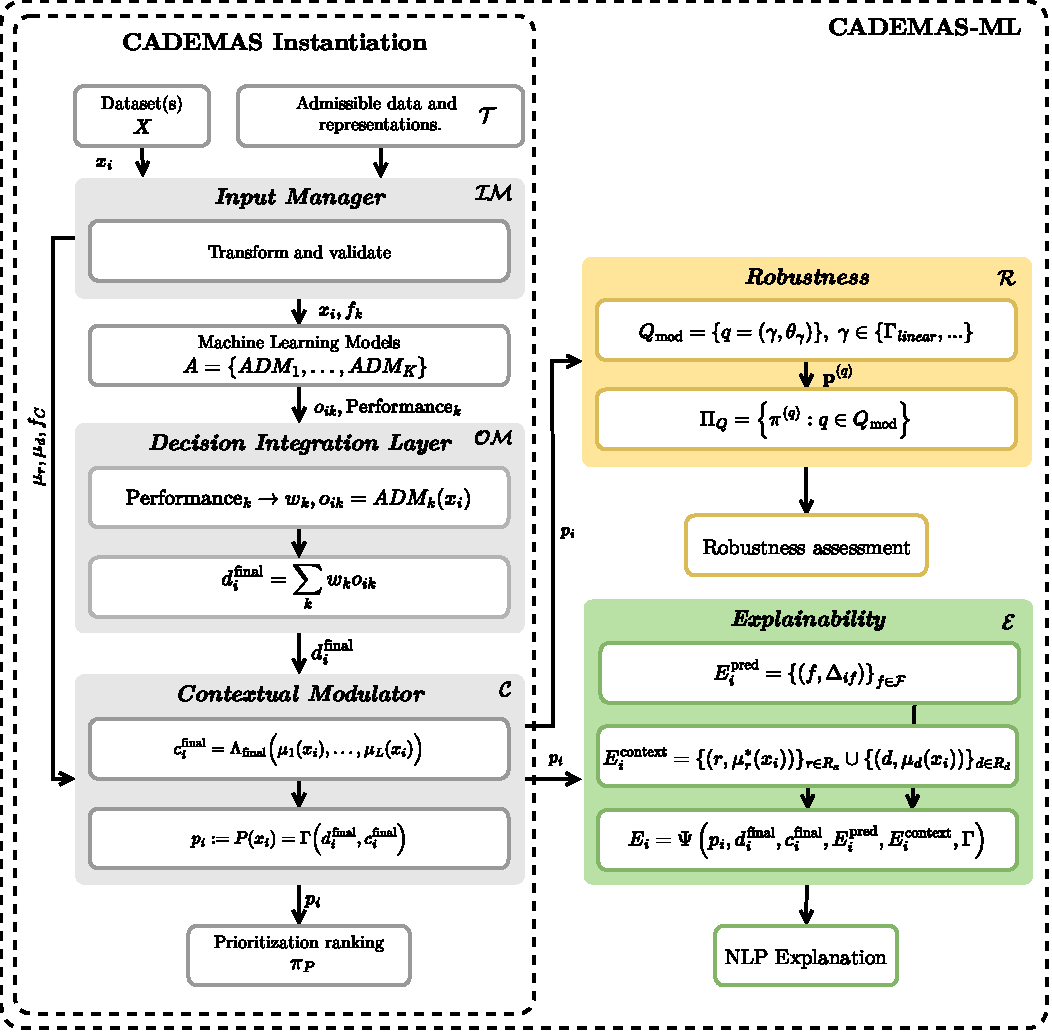
\includegraphics[width=\textwidth]{figures/instantiation.pdf}
    \caption{Specialization of the CADEMAS architecture for prioritization in CADEMAS-ML.}
    \label{fig:cademas_specialization}
\end{figure}

The following subsections formalize these components and introduce the explainability and robustness extensions added to the specialization. We denote these extensions by $\mathcal{E}$ and $\mathcal{R}$, respectively. Figure~\ref{fig:cademas_specialization} summarizes how each CADEMAS component is specialized for prioritization in CADEMAS-ML and how the two extensions complement the resulting decision process.

\subsection{Input Manager, ADM Units and Data Representation}\label{sec:input_manager}

The Input Manager $\mathcal{IM}$ coordinates the information required to configure and execute a prioritization process. In accordance with the general CADEMAS formulation, its role is to receive the relevant inputs, validate their consistency, and route them to the components that require them. For the purposes of the present formulation, the collection of ADM units and the set of cases are therefore treated as inputs coordinated by $\mathcal{IM}$ rather than as components of its internal representation.

Let
\begin{equation*}
A=\{ADM_1,\ldots,ADM_n\}
\end{equation*}
denote the collection of pre-trained machine-learning ADM units. Each $ADM_k$ provides a partial predictive assessment of the cases and may rely on a different subset of the available features. Let
\begin{equation*}
X=\{x_1,\ldots,x_N\}
\end{equation*}
denote the set of cases to be prioritized. Each case is represented by a set of observable features sufficient to satisfy the input requirements of the configured ADM units and contextual definition. In particular,
\begin{equation*}
f(x_i) \supseteq
\left(\bigcup_{k=1}^{n} f_k\right)
\cup f_{\mathcal{C}},
\end{equation*}
where $f_k$ denotes the features required by $ADM_k$ and $f_{\mathcal{C}}$ denotes the features required by the contextual definition.

Other inputs are also required to configure and execute a particular prioritization process, including the specifications associated with the ADM units and the contextual component. To keep the formalization focused on the decision flow, these inputs are assumed to be available to the corresponding CADEMAS components and are not included explicitly in the representation above. Their concrete structure and role in the software architecture are described in Section~\ref{sec:architecture_features}, together with the main input and configuration requirements.

The data representation $\mathcal{T}$ encompasses the tabular case data and the structured information required by the ADM and contextual components. Although these elements may be defined as collections to support alternative configurations, each execution selects one collection of ADM units, one contextual definition, and one case dataset. The Input Manager validates that the selected inputs are compatible and that all features required by the configured ADM units and contextual component are present and mutually consistent before the prioritization process is executed.


\subsection{Decision Integration Layer}\label{sec:decision_integration_layer}

The Decision Integration Layer ($\mathcal{OM}$) synthesizes the individual ADM outputs into the predictive score. In the present prioritization setting, each $ADM_k\in\mathcal{A}$ corresponds to a predictive model and produces a partial decision signal for case $x_i$:

\begin{equation*}
o_{ik}=ADM_k(x_i), \qquad o_{ik}\in[0,1],
\end{equation*}
where $o_{ik}$ denotes the output produced by the $k$-th predictive model for case $x_i$. For each case, let

\begin{equation*}
O_i=\{o_{i1},\ldots,o_{in}\}
\end{equation*}
denote the collection of model outputs associated with $x_i$.

To account for differences in predictive performance, each ADM unit is assigned a non-negative weight $w_k$, with

\begin{equation*}
w_k\geq0,
\qquad
\sum_{k=1}^{n}w_k=1.
\end{equation*}

The integrated decision signal for case $x_i$ is then obtained as

\begin{equation*}
d_i^{\mathrm{final}}
=
\Phi(O_i)
=
\sum_{k=1}^{n}w_k o_{ik},
\label{eq:integrated_decision}
\end{equation*}
where $d_i^{\mathrm{final}}\in[0,1]$ is the integrated predictive score for case $x_i$. In the present prioritization setting, this value represents the combined predictive signal before contextual modulation and is subsequently passed to the Contextual Modulator. 
The weights are derived from reported predictive performance. Integration operates directly on the outputs of the predictive models without modifying the models themselves, allowing heterogeneous predictors to contribute to a common predictive representation.
The predictive models may have been developed independently, using different training data, feature subsets, algorithms, or predictive objectives. Their combination therefore takes place at the decision level through the integration of their outputs.

\subsection{Contextual Modulator}\label{sec:contextual_modulator}

The Contextual Modulator \(\mathcal{C}\) represents contextual conditions through a declarative fuzzy specification. Following the role of context in \citet{NovoaHernandez2026} and the use of fuzzy propositions in the attrition application of \citet{Godz2026}, each context definition specifies the case attributes to be considered, the corresponding fuzzy propositions, and the aggregation rules used to obtain a contextual assessment. 

Formally, let \(V_r\) denote a case attribute and \(\tilde{F}_r\) a fuzzy set representing a linguistic predicate over the universe of \(V_r\). For case \(x_i\), an \textit{atomic contextual rule} evaluates the proposition ``\(V_r\) is \(\tilde{F}_r\)'' as

\begin{equation}
\mu_r(x_i)=\mu_{\tilde{F}_r}(x_{ir})\in[0,1],
\label{eq:atomic_mu}
\end{equation}
where \(x_{ir}\) is the value of \(V_r\) for case \(x_i\). The supported numerical and categorical membership functions, including triangular, trapezoidal, and linear forms, are specified in Appendix~\ref{app:context_math_mf}.

Atomic rules may also include activation conditions. Let \(m_r(x_i)\in\{0,1\}\) indicate whether the \texttt{when} condition of rule \(r\) is satisfied for case \(x_i\). Its effective membership is then

\begin{equation}
\mu_r^{*}(x_i)=m_r(x_i)\mu_r(x_i),
\label{eq:conditional_mu}
\end{equation}
with \(m_r(x_i)=1\) for unconditional rules. This allows conditional policies to be expressed declaratively, without modifying the case data or introducing procedural logic.

Context definitions may further include \textit{derived rules} that combine previously evaluated memberships. For a derived rule \(d\), its membership is given by

\begin{equation}
\mu_d(x_i)=
\Lambda_d\left(
\mu_{r_1}^{*}(x_i),\ldots,\mu_{r_q}^{*}(x_i)
\right),
\label{eq:derived_mu}
\end{equation}
where \(\Lambda_d\) is an aggregation operator. The implemented operators (minimum-based \texttt{AND}, maximum-based \texttt{OR}, algebraic \texttt{PRODUCT}, and linear \texttt{AVERAGE}) are defined in Appendix~\ref{app:context_math_derived}. The contextual alignment score for case \(x_i\) is finally obtained as

\begin{equation}
c_i^{\mathrm{final}}=
\Lambda_{\mathrm{final}}\left(
\mu_1(x_i),\ldots,\mu_L(x_i)
\right),
\label{eq:context_score}
\end{equation}
where \(\Lambda_{\mathrm{final}}\) is the final aggregation policy specified by the context definition.

The resulting \(c_i^{\mathrm{final}}\) represents the degree to which case \(x_i\) satisfies the contextual conditions of the selected scenario. All atomic and derived memberships are retained by the tool, so the contextual assessment remains traceable to the underlying fuzzy rules.

\subsubsection{Contextual Modulation}

The contextual assessment \(c_i^{\mathrm{final}}\) is subsequently used by the Contextual Modulator \(\mathcal{C}\) to transform the ADM-branch score \(d_i^{\mathrm{final}}\) into the priority score \(p_i\). Within the freedom provided by the general formulation (Section~\ref{sec:cademas}), CADEMAS-ML instantiates this component with three alternative contextual modulation operators, following the analysis in \citet{novoa2026aggregation}: the weighted linear mean, the weighted geometric mean, and the minimum operator.

Let \(d_i^{\mathrm{final}}\in[0,1]\) denote the integrated predictive signal and \(c_i^{\mathrm{final}}\in[0,1]\) the contextual alignment score. The priority score is obtained by instantiating the priority function \(P\) as follows:
\begin{equation*}
p_i
:=
P(x_i)
=
\Gamma\left(
d_i^{\mathrm{final}},c_i^{\mathrm{final}}
\right),
\label{eq:contextual_modulation}
\end{equation*}
where \(\Gamma \in \{\Gamma_{\mathrm{linear}}, \Gamma_{\mathrm{geom}}, \Gamma_{\mathrm{min}}\}\) denotes the selected contextual modulation operator. Specifically, the weighted linear operator is defined as
\begin{equation}
\Gamma_{\mathrm{linear}}
\left(
d_i^{\mathrm{final}},c_i^{\mathrm{final}}
\right)
=
\lambda d_i^{\mathrm{final}}
+
(1-\lambda)c_i^{\mathrm{final}},
\qquad \lambda\in[0,1],
\label{eq:linear_modulation}
\end{equation}
which has been used in previous CADEMAS applications \citep{NovoaHernandez2026,Godz2026}. In contrast, the weighted geometric operator is given by
\begin{equation}
\Gamma_{\mathrm{geom}}
\left(
d_i^{\mathrm{final}},c_i^{\mathrm{final}}
\right)
=
\left(d_i^{\mathrm{final}}\right)^{\lambda}
\left(c_i^{\mathrm{final}}\right)^{1-\lambda}, \qquad \lambda\in[0,1],
\label{eq:geometric_modulation}
\end{equation}
whereas the minimum operator is defined as
\begin{equation}
\Gamma_{\min}
\left(
d_i^{\mathrm{final}},c_i^{\mathrm{final}}
\right)
=
\min\left\{
d_i^{\mathrm{final}},c_i^{\mathrm{final}}
\right\}.
\label{eq:min_modulation}
\end{equation}

The linear operator allows compensation between predictive and contextual evidence, while the geometric and minimum operators impose more restrictive forms of cooperation. The parameter \(\lambda\) controls the relative contribution of the two sources for the linear and geometric operators; the minimum operator is parameter-free.

\subsection{Explainability Extension}\label{sec:explainability}

CADEMAS-ML extends the prioritization workflow with a case-level explanation mechanism, denoted by $\mathcal{E}$, that makes the cooperative decision process inspectable. It combines two complementary sources of evidence: a predictive explanation that estimates the local influence of input features on $d_i^{\mathrm{final}}$, and a contextual explanation that traces $c_i^{\mathrm{final}}$ back to the fuzzy evidence used in its assessment.

For a selected case $x_i$, the explanation also preserves the relation between the predictive and contextual components and the resulting priority score. The values $d_i^{\mathrm{final}}$ and $c_i^{\mathrm{final}}$ are reported together with the selected contextual modulation operator $\Gamma$. Depending on the operator, the explanation can therefore show the compensatory contribution of both components or identify the component limiting the final score.

The predictive component is explained through a model-agnostic perturbation procedure suitable for the heterogeneous and potentially ensemble-based ML models supported by the tool. For each ADM unit $ADM_k$ and feature $f$, the local effect is estimated by comparing the original prediction with the prediction obtained after replacing the observed feature value with a cohort reference value $b_f$:
\begin{equation*}
\Delta_{ikf}
=
ADM_k(x_i)-ADM_k\left(x_i^{(f\leftarrow b_f)}\right),
\label{eq:local_attribution_model}
\end{equation*}
where $b_f$ is the median of the reference cohort for numerical features and the mode for categorical features. The ADM-specific effects are then integrated using the same weights employed by the Decision Integration Layer:
\begin{equation*}
\Delta_{if}
=
\sum_{k=1}^{n}w_k\Delta_{ikf}.
\label{eq:local_attribution_global}
\end{equation*}
Positive values indicate that the observed feature value increases the integrated predictive score relative to the reference value, whereas negative values indicate a decrease. These quantities represent approximate local feature effects and should not be interpreted as causal estimates. The predictive explanation is represented as
\begin{equation*}
E_i^{\mathrm{pred}}
=
\left\{
(f,\Delta_{if})
\right\}_{f\in F},
\label{eq:predictive_explanation}
\end{equation*}
where $F$ denotes the set of features considered in the perturbation analysis.

The contextual component is traced back to the fuzzy propositions and derived rules defined in the selected context. By retaining the membership values of the evaluated rules, the tool exposes the intermediate evidence underlying the contextual assessment:
\begin{equation*}
E_i^{\mathrm{context}}
=
\left\{
(r,\mu_r^*(x_i))
\right\}_{r\in R_a}
\cup
\left\{
(d,\mu_d(x_i))
\right\}_{d\in R_d},
\label{eq:context_explanation}
\end{equation*}
where $R_a$ and $R_d$ denote the sets of atomic and derived rules evaluated for case $x_i$, respectively. The use of $\mu_r^*(x_i)$ for atomic rules accounts for possible activation conditions.

The two sources of evidence are finally combined into a deterministic natural-language representation. For case $x_i$, the resulting explanation can be expressed as
\begin{equation*}
E_i =
\Psi\left(
p_i,
d_i^{\mathrm{final}},
c_i^{\mathrm{final}},
E_i^{\mathrm{pred}},
E_i^{\mathrm{context}},
\Gamma
\right),
\label{eq:natural_language_explanation}
\end{equation*}
where $\Gamma$ denotes the selected contextual modulation operator, including its parameterization when applicable. The function $\Psi$ translates these intermediate results into a structured textual account of the predictive and contextual factors underlying the final prioritization.

\subsection{Robustness Extension}\label{sec:robustness}

As anticipated in Section~\ref{sec:intro}, the robustness extension, denoted by $\mathcal{R}$, evaluates the stability of prioritization results under alternative contextual modulation configurations. Let
\[
Q_{\mathrm{mod}}
=
\left\{
q=(\gamma,\theta_\gamma)
\right\},
\qquad
\gamma\in
\{\Gamma_{\mathrm{arith}},\Gamma_{\mathrm{geom}},\Gamma_{\min}\},
\]
denote the set of configurations explored by the analyst, where $\gamma$ identifies the selected modulation operator and $\theta_\gamma$ its associated parameterization, which may be empty for parameter-free operators. Each configuration $q\in Q_{\mathrm{mod}}$ induces a priority score vector
\[
\mathbf{p}^{(q)}
=
\left(
p_1^{(q)},\ldots,p_N^{(q)}
\right),
\qquad
p_i^{(q)}:=P^{(q)}(x_i),
\]
and an associated ranking $\pi^{(q)}$ over the cases.

Within-operator robustness examines the effect of changing the parameterization while keeping the modulation operator fixed. For the arithmetic and weighted geometric operators, the analyst can explore different values of $\lambda$ and compare the resulting scores and rankings. The parameter-free minimum operator can be included as a reference configuration.

Across-operator robustness examines the effect of changing the contextual modulation operator while keeping the predictive and contextual signals fixed. The available operators,
\[
\{\Gamma_{\mathrm{arith}},\Gamma_{\mathrm{geom}},\Gamma_{\min}\},
\]
may produce different scores and rankings. Their comparison allows the analyst to identify cases whose prioritization remains stable across operators and cases whose position is sensitive to the selected modulation mechanism.

More generally, the tool considers the collection
\[
\Pi_{Q}
=
\left\{
\pi^{(q)}:q\in Q_{\mathrm{mod}}
\right\}
\]
of rankings induced by the explored configurations. These rankings can be inspected individually or jointly, allowing within-operator and across-operator comparisons to be performed independently or in combination.

The robustness analysis does not assume a universally preferred modulation operator. Instead, it reveals the extent to which prioritization outcomes depend on the parameterization of a given operator and on the choice of modulation mechanism.


\section{Architecture and main functionalities}\label{sec:architecture_features}\label{sec:results}

Once the CADEMAS instantiation for prioritization has been defined and formalized, the present section describes how it is realized as an executable software workflow. The software architecture is first presented, followed by its main functionalities and their illustration through an employee-attrition case study.

\subsection{Software architecture}\label{sec:software_arch} 

CADEMAS-ML is implemented as a Python application based on Streamlit \citep{streamlit}, providing an interactive interface for configuring, executing, and inspecting the prioritization process. The architecture follows the structure introduced in Section~\ref{sec:instantiation}, while keeping the computational components independent from the interface. Predictive inference relies on H2O \citep{H2O.ai2026} MOJO artifacts, allowing independently trained models with heterogeneous feature subsets to be loaded at run time without requiring the original training code. Contextual evaluation is performed by a vectorized fuzzy engine that reads declarative JSON specifications, allowing alternative contextual definitions to be evaluated without modifying the application logic. Interactive visualizations are generated with Altair \citep{VanderPlas2018} and integrated into the corresponding inspection views.

\begin{figure}[!t]
    \centering
    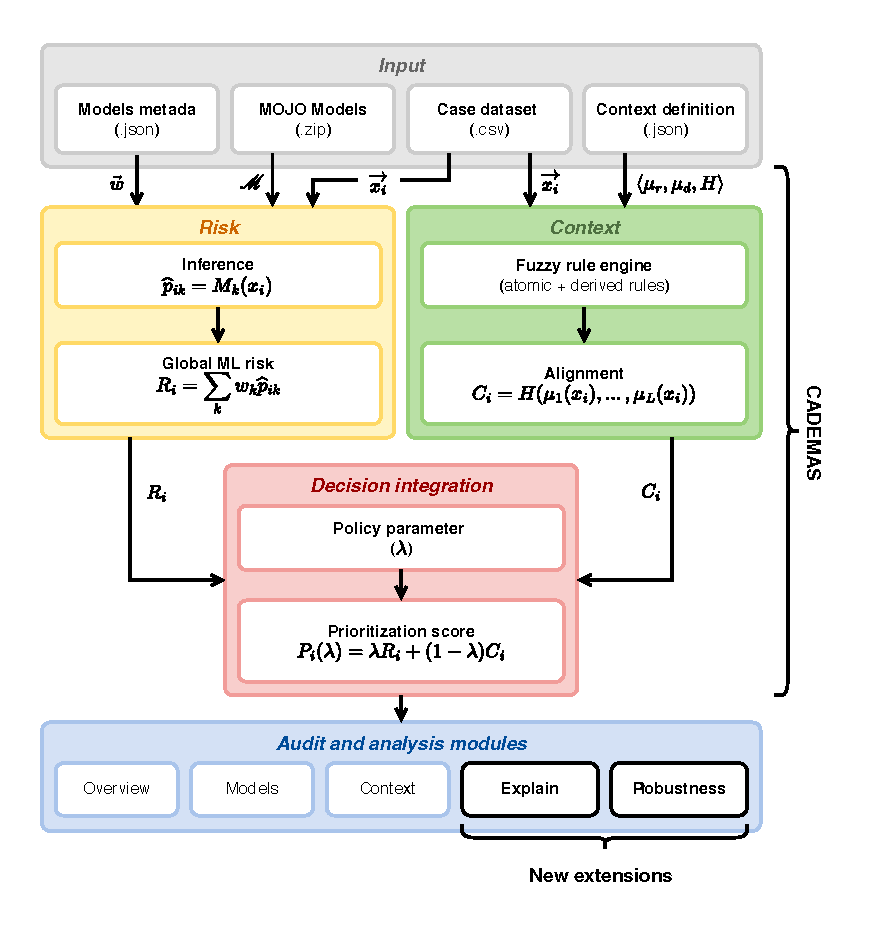
\includegraphics[width=\textwidth]{figures/architecture.pdf}
    \caption{Architecture of CADEMAS-ML as a Streamlit application. Four inputs feed an \textit{Inputs and Parameter Settings} stage (validation and preprocessing), followed by a \textit{Prioritization engine} that implements decision integration and contextual modulation. The resulting scores are inspected through five views: \textit{Overview}, \textit{Models}, \textit{Context}, \textit{Explain}, and \textit{Robustness}.}
    \label{fig:software_architecture}
\end{figure}

Figure~\ref{fig:software_architecture} summarizes the resulting workflow. A run requires a model-metadata JSON file, one or more context JSON files, the corresponding MOJO models, and a tabular case dataset. The \textit{Inputs and Parameter Settings} stage validates and prepares these inputs and allows the analyst to configure the main parameters of the prioritization process. These include the performance metric used to derive model weights, the fuzzy aggregation used to obtain the contextual alignment score, the contextual modulation operator (e.g. linear, geometric, or minimum), and, when applicable, the balance parameter $\lambda$.

The prepared inputs are then passed to the \textit{Prioritization engine}, which implements the Decision Integration Layer and the Contextual Modulator described in Section~\ref{sec:instantiation}. The predictive model outputs are first combined into an integrated predictive score. The contextual component then evaluates the selected fuzzy definitions to obtain the contextual alignment score. Finally, the selected modulation operator combines both signals to produce the priority score for each case.

The resulting information is exposed through the \textit{Overview}, \textit{Models}, \textit{Context}, \textit{Explain}, and \textit{Robustness} views. These views allow the analyst to inspect the intermediate and final results, examine individual cases, trace the predictive and contextual evidence behind their scores, and assess the stability of the resulting prioritization. 

%In CADEMAS terms, the application operationalizes $\mathcal{IM}$, the predictive ADM units, $\mathcal{OM}$, and $\mathcal{C}$, together with the explainability and robustness extensions $\mathcal{E}$ and $\mathcal{R}$.


\subsection{Main functionalities}\label{sec:main_functionalities}

To illustrate the main functionalities of CADEMAS-ML, we use an employee-attrition case study and describe how the different stages of the prioritization process are configured and executed. The example uses the employee-attrition configuration distributed with the repository and follows the workflow presented in Figure~\ref{fig:software_architecture}. Its purpose is to illustrate how heterogeneous predictive assessments and explicit contextual policies can be integrated, inspected, and explained within the proposed architecture.


\subsubsection{Employee-attrition case study}\label{sec:demo_setup}

The case study considers an organization that must prioritize employee-retention interventions under limited resources. Predictive information is provided by four organizational perspectives: Culture and Wellbeing, Finance, Operations and Development, and Human Resources. Each perspective is represented by an independently trained model using a different subset of employee attributes from the same workforce records. This setting represents a decision process in which different organizational units contribute partial predictive assessments based on the information relevant to their respective perspectives.

All models were trained offline using the publicly available IBM HR Analytics Employee Attrition and Performance dataset \citep{IBMHRKaggle}. The dataset contains 1{,}470 employee records and 35 attributes covering demographic, professional, compensation, performance, and organizational characteristics. Following \citet{Godz2026}, H2O AutoML was applied independently to each feature subset defined in Appendix~\ref{app:attrition_features}, using an 80/20 train--validation partition and a one-hour time budget for each model. The resulting MOJO artifacts, validation metrics, and feature assignments are distributed with the application.

Contextual information is specified independently from the predictive models through JSON-based fuzzy specifications. The example bundle contains two organizational policies, \textit{Economic Crisis} and \textit{Digital / Technological Transformation}. Both policies use the same predictive layer but define different contextual conditions. The present case study focuses on \textit{Digital / Technological Transformation}, whose contextual assessment considers upskilling capacity, role adaptability, career scalability, and investment horizon in the context of a technological-change program. The corresponding specification is provided in Appendix~\ref{app:context_specs}.

For interactive demonstration, the repository includes a 20-case CSV subset containing the same predictors as the original dataset, together with the \texttt{attrition} outcome label. This label is retained for verification purposes but is not used to compute the prioritization scores. The values in \texttt{Case\_ID} are randomly generated identifiers used to reference cases in the application and throughout the analysis. Unless otherwise stated, the results presented below correspond to the Linear modulation operator with $\lambda=0.5$.

\begin{figure}[!t]
	\centering
	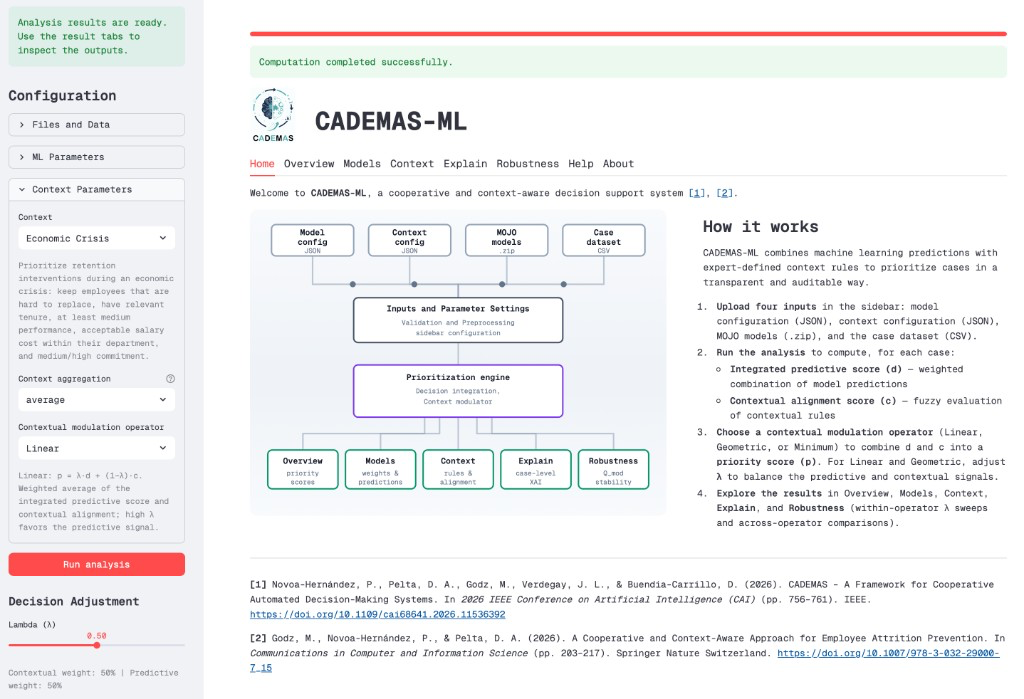
\includegraphics[width=\textwidth]{figures/home.png}
	\caption{\textit{Home} view of CADEMAS-ML after a completed run. The sidebar exposes context selection, fuzzy aggregation, the contextual modulation operator, and $\lambda$; the main panel summarizes the prioritization workflow shown in Figure~\ref{fig:software_architecture}.}
	\label{fig:home_upload}
\end{figure}

The analysis is initiated from the \textit{Home} view and its sidebar upload controls (Figure~\ref{fig:home_upload}). The analyst provides the model-metadata JSON, context JSON, MOJO models, and case dataset, or alternatively loads the ready-made configuration from \texttt{example\_attrition/}. The performance metric, context specification, fuzzy aggregation, contextual modulation operator, and, when applicable, $\lambda$ are then selected before \textit{Run analysis} executes the prioritization workflow. Table~\ref{tab:tool_model_weights} reports the four pre-trained models and the AUC-based weights computed during the run. The lower validation AUC of the Operations and Development model results in a correspondingly lower weight than those assigned to the other three models.

\begin{table}[!th]
	\centering
\tbl{Models used in the attrition example and AUC-based weights computed by CADEMAS-ML. The \textit{AutoML model} column summarizes the artifact exported by H2O AutoML.}
{\begin{tabularx}{\textwidth}{lllcc}
\toprule
\textbf{ID} & \textbf{Organizational perspective} & \textbf{AutoML model} & \textbf{AUC} & \textbf{Weight} \\
\midrule
$M_1$ & Culture and Wellbeing & Stacked Ensemble (BestOfFamily) & 0.9941 & 0.2623 \\
$M_2$ & Finance & Stacked Ensemble (BestOfFamily) & 0.9972 & 0.2631 \\
$M_3$ & Operations and Development & GBM (grid 1, model 26) & 0.8022 & 0.2116 \\
$M_4$ & Human Resources & Stacked Ensemble (BestOfFamily) & 0.9968 & 0.2630 \\
\bottomrule
\end{tabularx}}
\label{tab:tool_model_weights}
\end{table}


\subsubsection{Integrated prioritization overview}\label{sec:func_overview}

After execution, the \textit{Overview} module presents the integrated predictive score, the contextual alignment score, and the resulting priority score for each case. Figure~\ref{fig:overview} shows the interface for the \textit{Digital / Technological Transformation} context under Linear modulation with $\lambda=0.5$. The scatter plot represents the cases in the predictive--contextual score space and uses the priority score to distinguish their final assessment. The adjacent histogram shows the distribution of priority scores across the cohort. The table below lists all cases in priority order and reports the two component scores together with the \texttt{attrition} label, which is retained for verification only. In this run, contextual alignment ranges from 0.1500 to 0.7100, with a mean of 0.4663. The ten highest-priority cases are considered again in the robustness analysis presented in Figure~\ref{fig:robustness}.

\begin{figure*}[!tb]
\centering
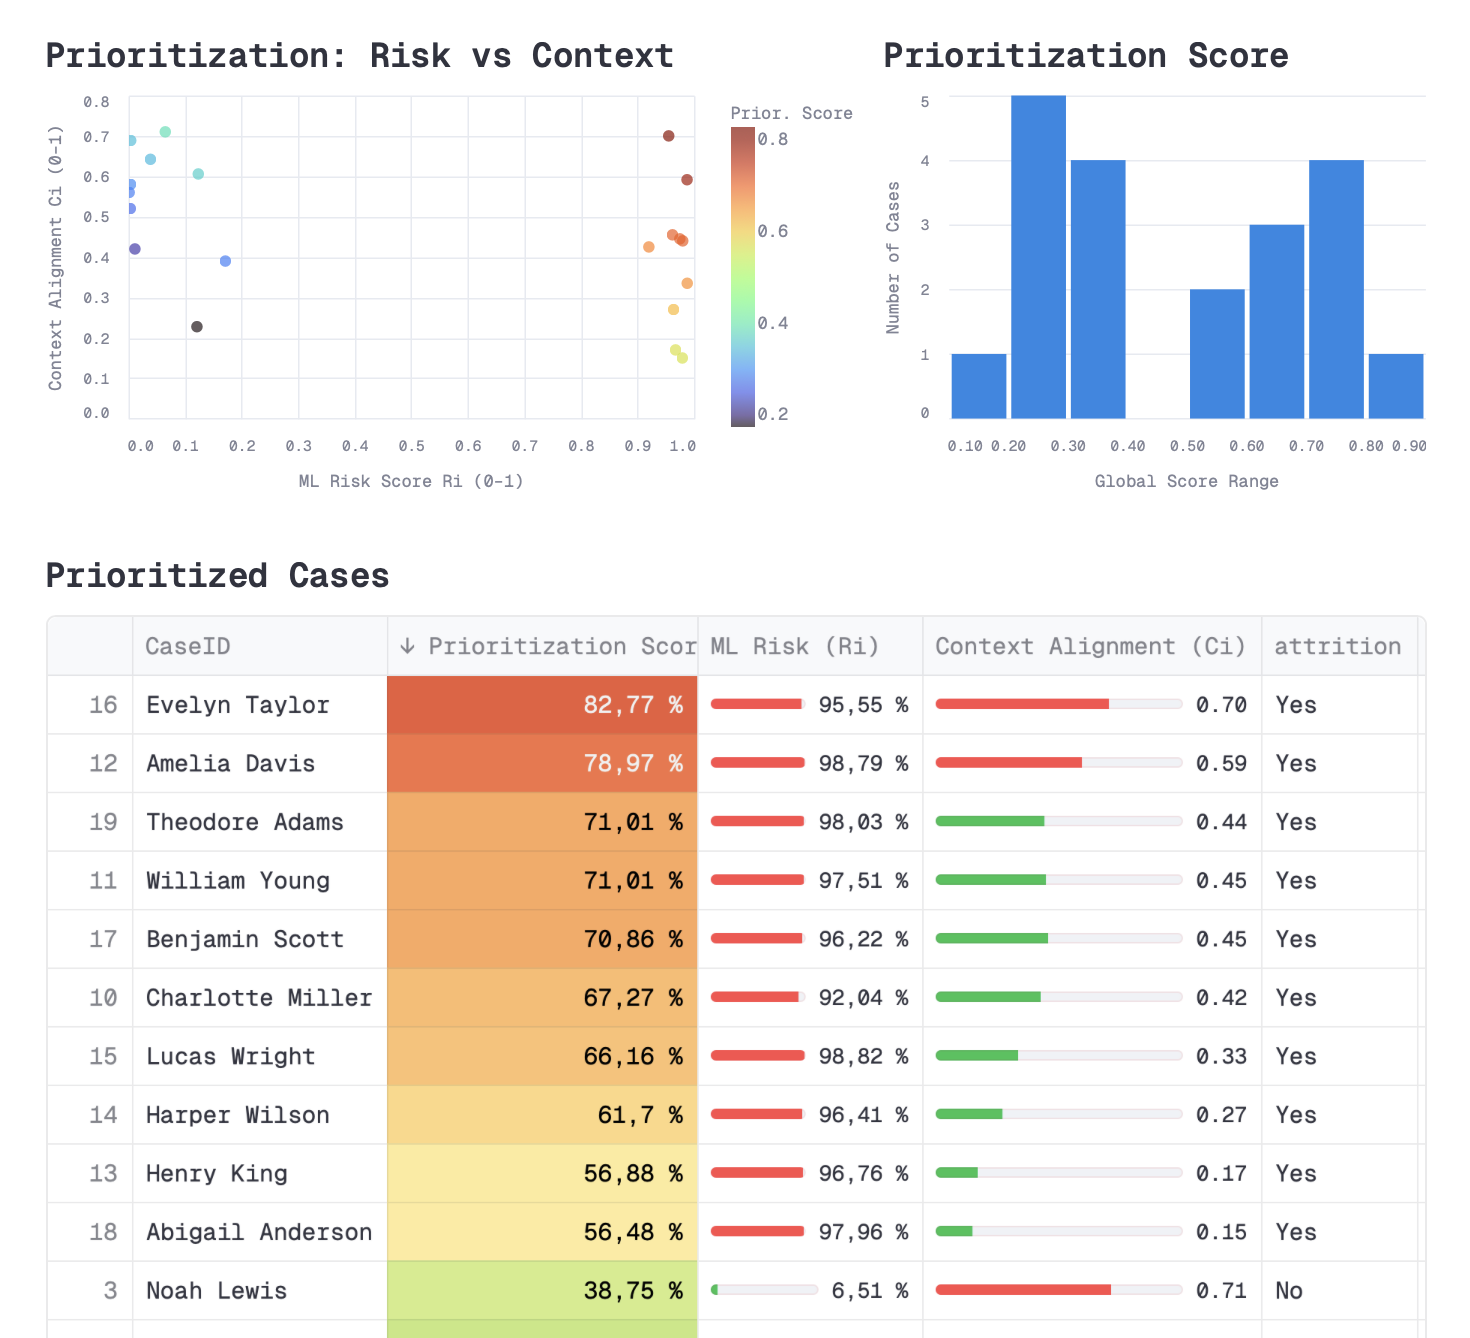
\includegraphics[width=\textwidth]{figures/overview.png}
\caption{\textit{Overview} module for the attrition example under Linear modulation with $\lambda=0.5$ in the \textit{Digital / Technological Transformation} context. The scatter plot and histogram summarize the predictive and contextual scores and the resulting priority distribution, while the table lists the complete cohort in priority order.}
\label{fig:overview}
\end{figure*}

The resulting ranking illustrates how the two components jointly determine the final prioritization. \textit{Evelyn Taylor} receives the highest priority, with a predictive score of $0.9555$ and a contextual alignment of $0.7000$. Other cases, such as \textit{Lucas Wright} and \textit{Abigail Anderson}, also occupy high positions because of their elevated predictive scores, despite having more moderate contextual alignment. The opposite situation is illustrated by \textit{Noah Lewis}, who has the highest contextual alignment in the cohort ($0.7100$) but a low integrated predictive score ($0.0651$). Under $\lambda=0.5$, these values result in a priority score of $0.3875$, placing the case well below the highest-priority positions. The joint presentation of the two components and the resulting score therefore makes the effect of contextual information visible without treating contextual alignment itself as the prioritization criterion.


\subsubsection{Inspecting the integrated predictive score}\label{sec:func_models}

The \textit{Models} module exposes the Decision Integration Layer. Figure~\ref{fig:models} shows the corresponding interface for the run presented above. The upper table associates each uploaded MOJO with the selected performance metric and its normalized weight $w_k$, consistent with the values reported in Table~\ref{tab:tool_model_weights}. The lower table reports the positive-class probability produced by each model for every case, together with the resulting integrated predictive score. Cases are ordered by decreasing integrated score.

\begin{figure*}[!tb]
\centering
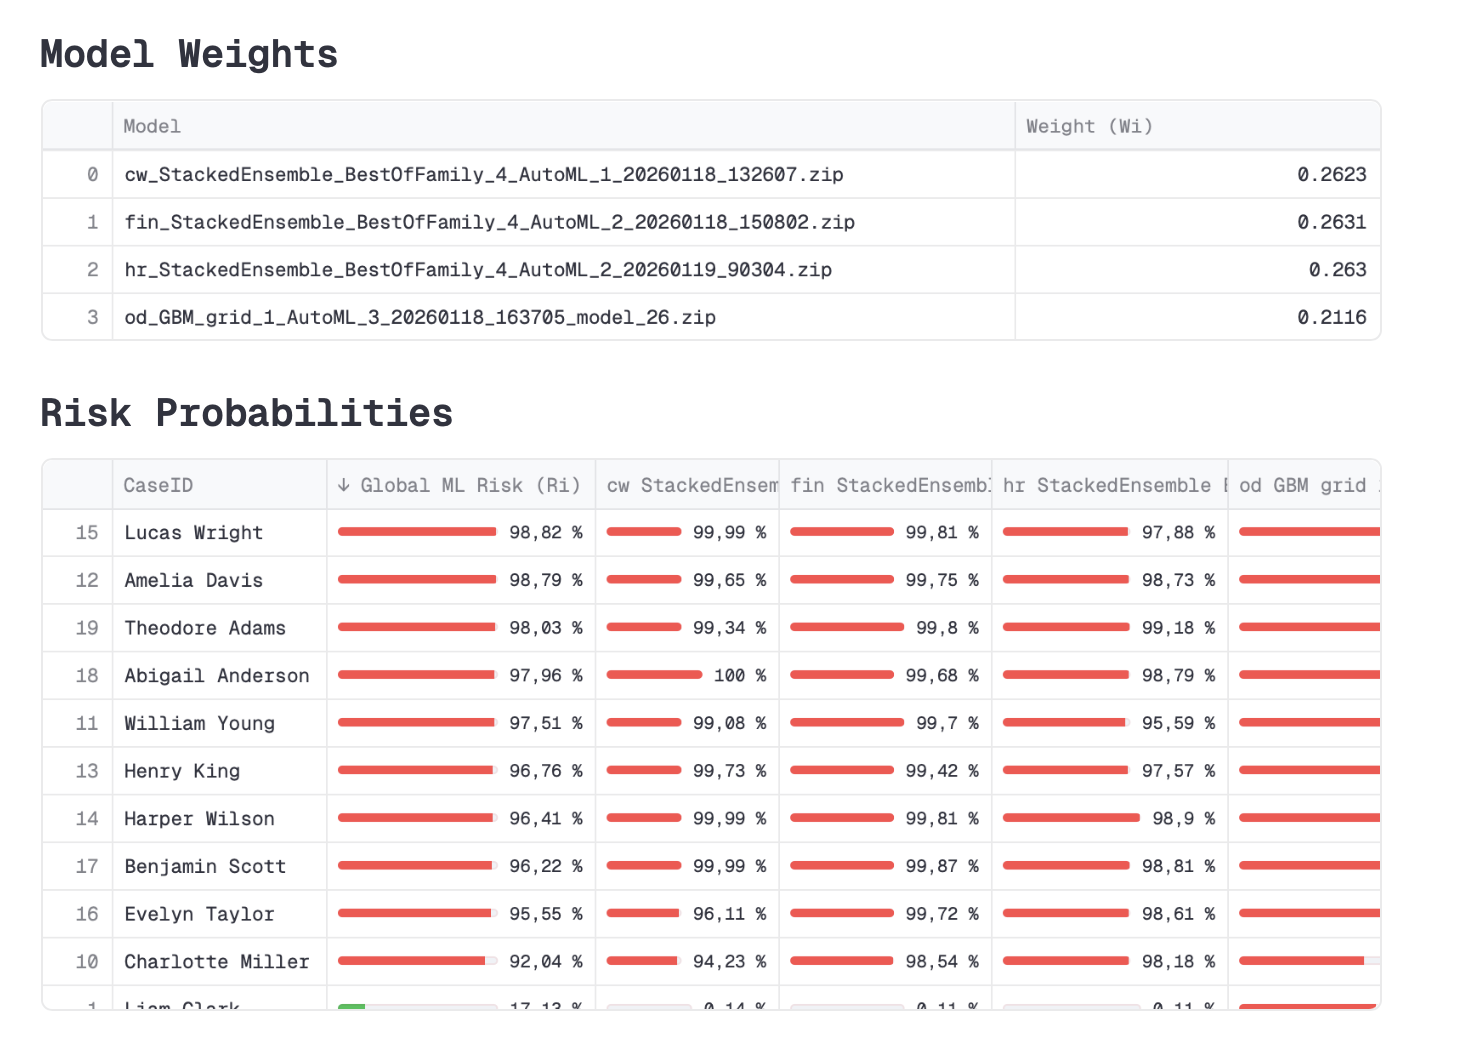
\includegraphics[width=\textwidth]{figures/models.png}
\caption{\textit{Models} module for the attrition example. The upper table reports the performance metric and contribution weight $w_k$ of each MOJO, while the lower table shows the per-model predictions and the resulting integrated predictive score, with cases ordered by decreasing integrated score.}
\label{fig:models}
\end{figure*}

In the exported view, \textit{Lucas Wright} ranks first with an integrated score of $0.9882$, followed by \textit{Amelia Davis} ($0.9879$) and \textit{Theodore Adams} ($0.9803$). This ordering reflects the predictive layer alone and differs from the prioritization ranking in Figure~\ref{fig:overview}, where \textit{Evelyn Taylor} receives the highest priority after contextual alignment is incorporated. The per-model prediction columns also make the integration process transparent. Although all four MOJOs assign high attrition probabilities to the top-ranked cases, the Operations and Development model has a smaller contribution to the integrated score because of its lower validation weight ($w_3=0.2116$).

\subsubsection{Contextual alignment evaluation}\label{sec:func_context}

The \textit{Context} module exposes the fuzzy evaluation underlying the contextual alignment score. Figure~\ref{fig:context} shows the interface for the \textit{Digital / Technological Transformation} context. The upper panel allows the analyst to select an atomic rule and inspect its membership function together with the distribution of the corresponding feature across the cohort. A numerical audit table reports the crisp input value and membership degree for each case. The lower panel summarizes the satisfaction degrees of the composite rules and the resulting alignment score for the full cohort.

\begin{figure*}[!tb]
\centering
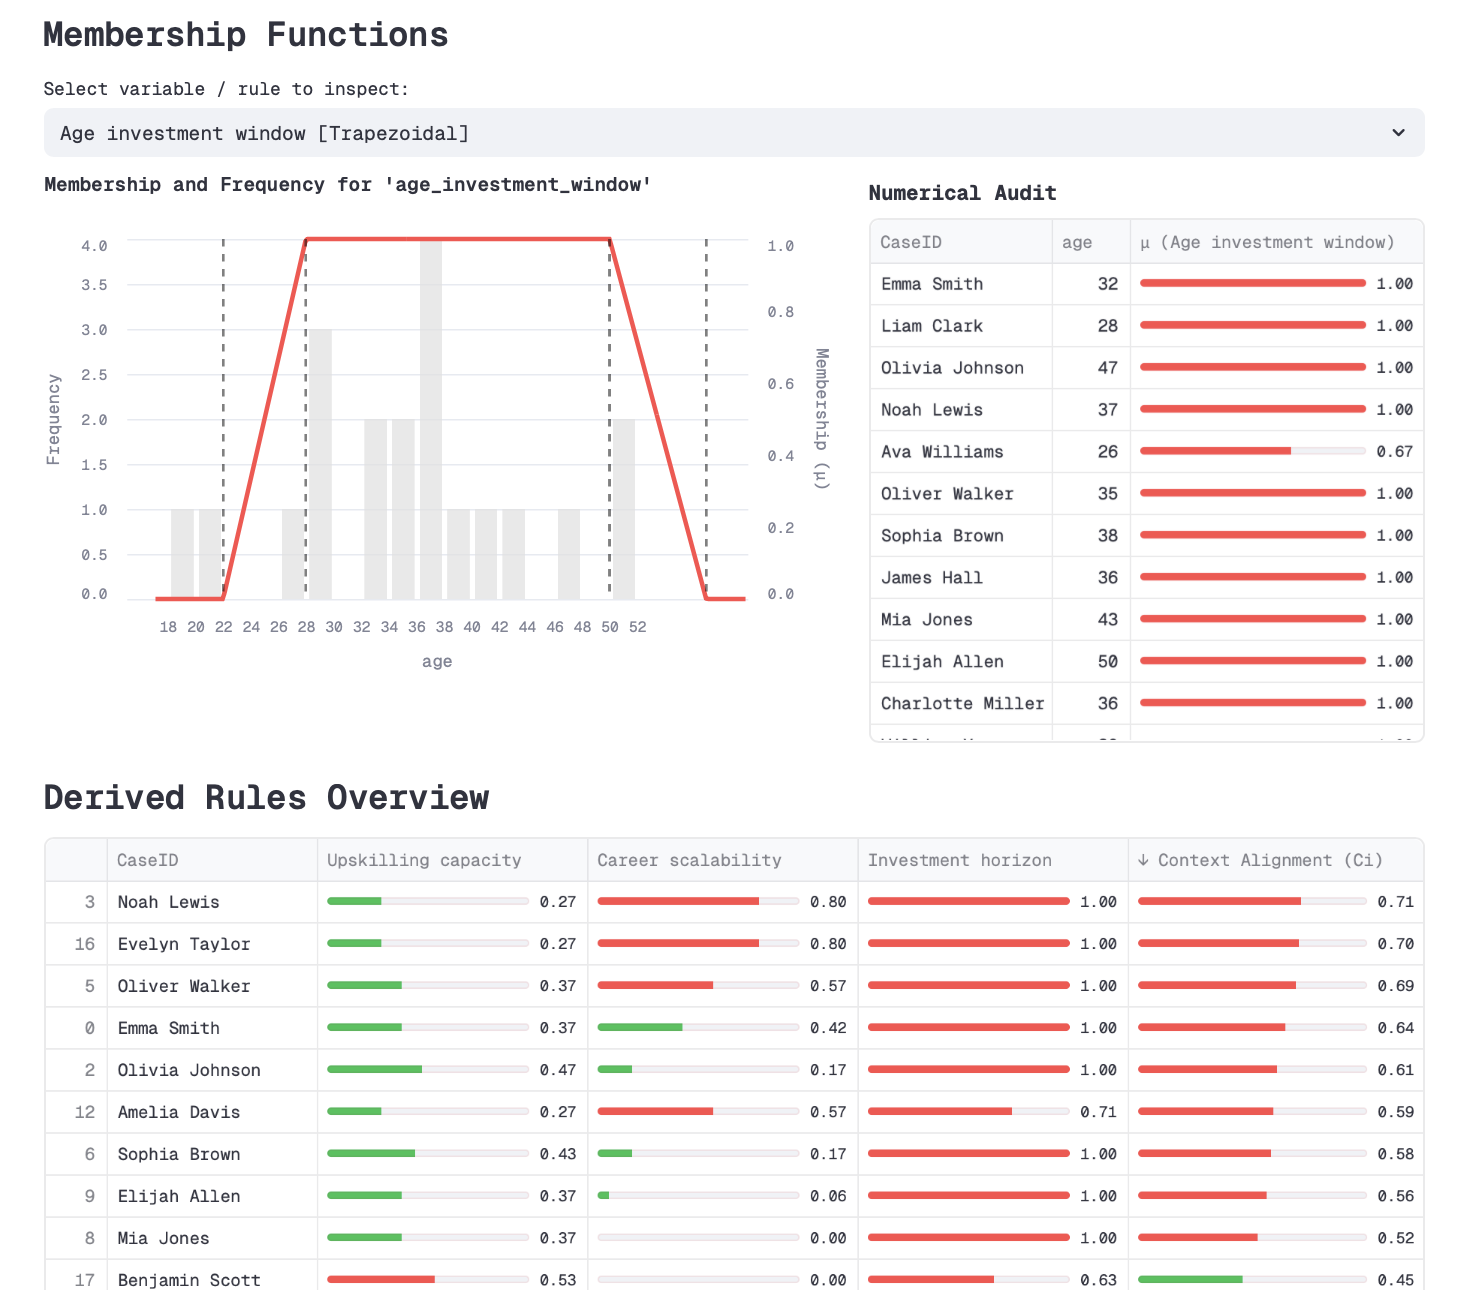
\includegraphics[width=\textwidth]{figures/context.png}
\caption{\textit{Context} module for the \textit{Digital / Technological Transformation} run. The interface combines an atomic-rule selector, the corresponding membership-function chart and case distribution, and a numerical audit for \textit{Age investment window}. The derived-rules overview reports membership degrees and contextual alignment for cases ordered by decreasing alignment.}
\label{fig:context}
\end{figure*}

In the exported view, the trapezoidal atomic rule \textit{Age investment window} defines the acceptable age range for developmental investment during the transformation program (Appendix~\ref{app:context_specs}). The chart shows how each employee's age maps to the corresponding membership degree, while the audit table reports the same evaluation numerically for each case. The derived-rules overview then reports the satisfaction degrees for \textit{Upskilling capacity}, \textit{Career scalability}, and \textit{Investment horizon}, together with the resulting contextual alignment score. When ordered by alignment, \textit{Noah Lewis} appears first ($0.7100$), followed by \textit{Evelyn Taylor} ($0.7000$), even though Evelyn receives the highest priority in Figure~\ref{fig:overview} because of her higher integrated predictive score. Across the cohort, contextual alignment ranges from $0.1500$ to $0.7100$. The \textit{Context} module therefore complements the global prioritization view by making the evidence underlying the contextual assessment auditable at both the rule and case levels.

\subsubsection{Case-level explanation}\label{sec:func_explain}

For a selected case, the \textit{Explain} module assembles the explanation layers described in Section~\ref{sec:explainability} into a single audit view. Figure~\ref{fig:explain} shows the interface for \textit{Evelyn Taylor}, the highest-priority case in Figure~\ref{fig:overview}. The upper panel provides the case selector, a deterministic natural-language summary, and the main statistics underlying that summary: priority score, integrated predictive score, contextual alignment, modulation operator, and $\lambda$ when applicable. Under Linear modulation, the relation between the two components and the resulting priority score has an additive interpretation; under Geometric or Minimum modulation, the same information reflects the corresponding multiplicative or limiting-factor effect. The lower panel reports aggregated predictive attributions for the most influential features and the fuzzy membership values that trace the degree to which each contextual rule is satisfied for the selected case.

\begin{figure*}[!tb]
\centering
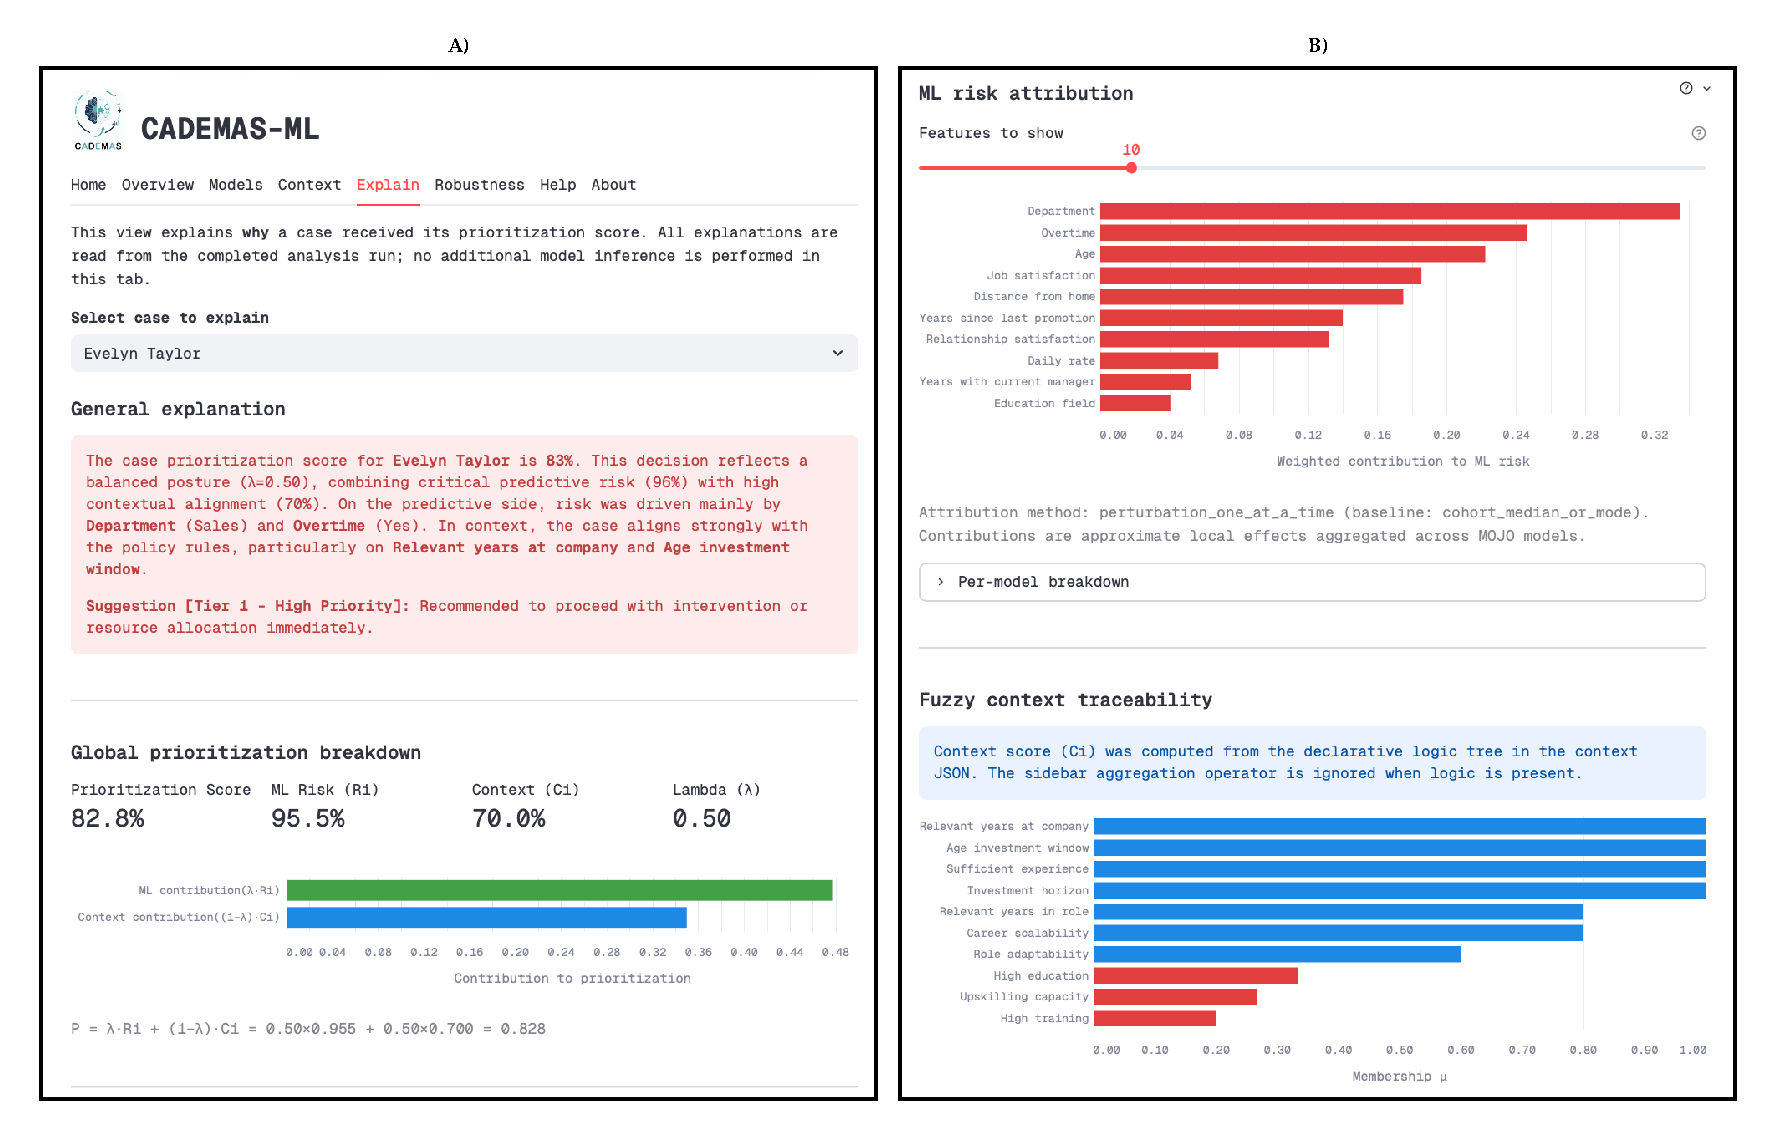
\includegraphics[width=\textwidth]{figures/explain_high_prioritization.pdf}
\caption{\textit{Explain} module for \textit{Evelyn Taylor} under Linear modulation with $\lambda=0.5$ in the \textit{Digital / Technological Transformation} context, with case selection, natural-language explanation, summary statistics, aggregated predictive feature attributions, and a fuzzy context-traceability panel.}
\label{fig:explain}
\end{figure*}

Two cases from the same run illustrate the interpretation provided at $\lambda=0.5$. The first is \textit{Evelyn Taylor}; the second is \textit{Noah Lewis}, who ranks low in the overview despite having the highest contextual alignment in the cohort. For space reasons, only the \textit{Evelyn Taylor} view is shown in the figure, while the contrasting \textit{Noah Lewis} summary is reported below. In both cases, the summaries follow the deterministic template implemented by the tool: the priority score is reported first, followed by the modulation configuration, the predictive and contextual scores, the main predictive drivers, the contextual rules that support or constrain the priority assessment, and a tier-based recommendation derived from the priority score.

\textit{Evelyn Taylor} combines a high integrated predictive score ($0.9555$) with high contextual alignment ($0.7000$), yielding a priority score of $0.8277$ and a Tier~1 recommendation. Figure~\ref{fig:explain} highlights Department (Sales) and Overtime (Yes) among the strongest predictive drivers and shows high membership on Relevant years at company and Age investment window in the fuzzy traceability panel:

\begin{quote}
\small
The case priority score for \textit{Evelyn Taylor} is 83\%. This decision reflects a balanced Linear modulation posture ($\lambda=0.50$), combining critical integrated predictive evidence (96\%) with high contextual alignment (70\%). On the predictive side, the signal was driven mainly by Department (Sales) and Overtime (Yes). In context, the case aligns strongly with the policy rules, particularly on Relevant years at company and Age investment window.

Suggestion [Tier 1 -- High Priority]: Recommended to proceed with intervention or resource allocation immediately.
\end{quote}

\textit{Noah Lewis} provides a contrasting interpretation. Although this case has the highest contextual alignment in the cohort ($0.7100$), its integrated predictive score is low ($0.0651$). The resulting priority score is therefore $0.3875$, and the module assigns Tier~3:

\begin{quote}
\small
The case priority score for \textit{Noah Lewis} is 39\%. This decision reflects a balanced Linear modulation posture ($\lambda=0.50$), combining low integrated predictive evidence (7\%) with high contextual alignment (71\%). On the predictive side, the signal was driven mainly by Years with current manager (8) and Number of companies worked (1). In context, the case aligns strongly with the policy rules, particularly on Relevant years at company and Age investment window.

Suggestion [Tier 3 -- Low Priority]: Intervention or resource allocation is not justified under current prediction and context guidelines.
\end{quote}

CADEMAS-ML therefore makes it possible to inspect not only why a case receives a high priority, but also why strong contextual alignment alone may not result in a high final score when the integrated predictive signal is limited. A third illustrative pattern is provided by \textit{Theodore Adams} (predictive score $0.9803$, alignment $0.4400$, priority score $0.7101$), who receives Tier~2 because the combination of high predictive evidence and moderate contextual alignment results in an intermediate priority under the current policy.

\subsubsection{Robustness and sensitivity analysis}\label{sec:func_robustness}

The \textit{Robustness} module implements the sensitivity analysis described in Section~\ref{sec:robustness}. The interface allows the analyst to assemble a set of modulation configurations $Q_{\mathrm{mod}}$ by selecting combinations of the Linear, Geometric, and Minimum operators. Shared $\lambda$ partitions apply to Linear and Geometric whenever these operators are included, whereas Minimum contributes a single parameter-free configuration. Cases displayed in the charts are the top $N$ under a selected configuration, by default the active operator at $\lambda\approx0.5$ or Minimum when it is the selected parameter-free option.

Figure~\ref{fig:robustness} illustrates the within-operator analysis for the \textit{Digital / Technological Transformation} run using the Linear operator only. The analysis therefore keeps the modulation mechanism fixed and varies $\lambda$ across the selected range. The bump chart traces priority ranks across these $\lambda$ configurations, the ranks box plot summarizes the rank distribution of each displayed case over the same configurations, and the rank acceptability indices estimate how often each case occupies each rank position. This analysis isolates the sensitivity of the prioritization to the relative contribution of predictive and contextual scores under a fixed modulation operator.

\begin{figure*}[!tb]
\centering
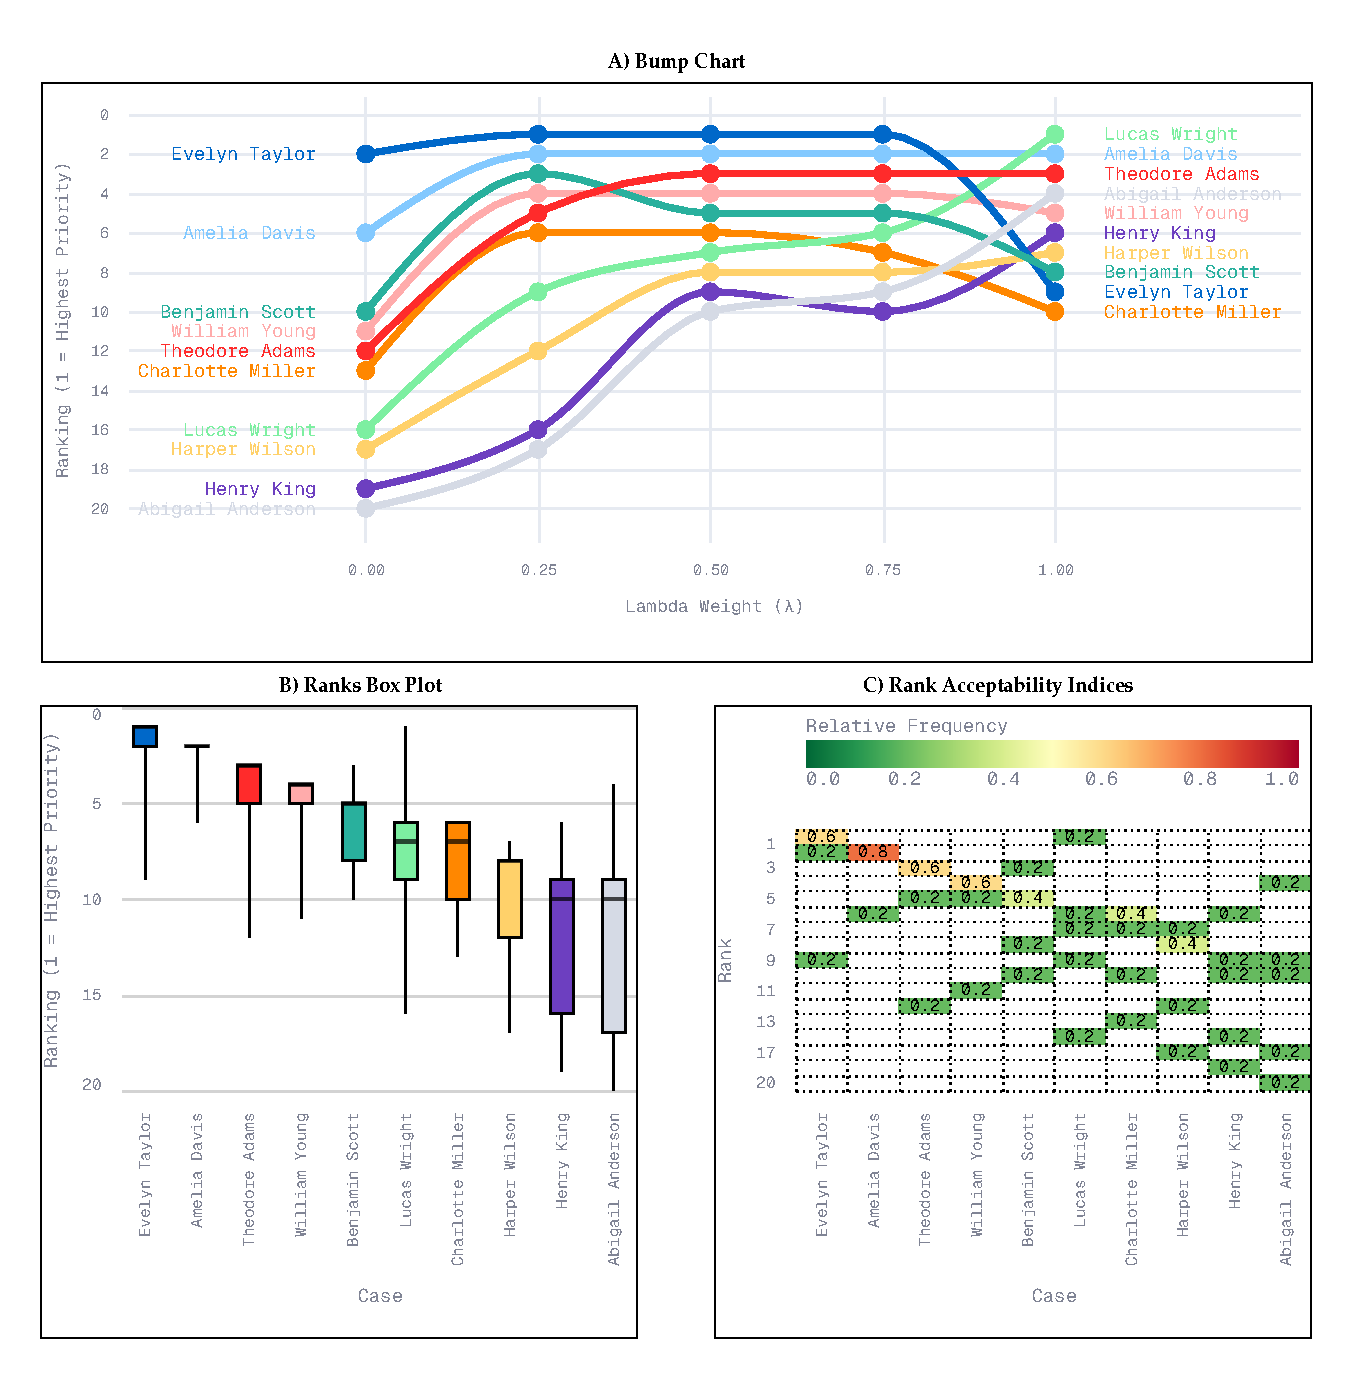
\includegraphics[width=\textwidth]{figures/robustness.pdf}
\caption{Within-operator robustness analysis for the \textit{Digital / Technological Transformation} context under the Linear modulation operator. The views summarize priority-rank trajectories, rank distributions, and rank acceptability indices over the selected $\lambda$ configurations for the top cases under the selected Top-$N$ configuration.}
\label{fig:robustness}
\end{figure*}

In the Linear $\lambda$-sweep illustrated in the figure, cases outside the top ten at $\lambda=0.5$, such as \textit{Noah Lewis} and \textit{Emma Smith}, rise in the ranking as greater weight is assigned to contextual alignment because they combine relatively high alignment with low integrated predictive scores. Conversely, when the predictive component receives greater weight, cases near the top of Figure~\ref{fig:overview}, such as \textit{Lucas Wright} and \textit{Theodore Adams}, retain high positions because of their elevated predictive scores. \textit{Evelyn Taylor} remains near the top across intermediate values of $\lambda$ because both component scores are high. Compact rank distributions indicate stable priorities across the explored configurations, whereas wider distributions identify cases whose position is more sensitive to the selected balance between predictive and contextual evidence.

The analysis shown here is therefore an intra-operator sensitivity analysis. The same functionality can also be used to perform across-operator comparisons by including configurations from different modulation operators in $Q_{\mathrm{mod}}$, but such comparisons are not included in the present case-study illustration.

\section{Conclusion and future work}\label{sec:discussion}

This paper presented CADEMAS-ML as a software tool that operationalizes the CADEMAS framework for cooperative, context-aware prioritization based on heterogeneous machine-learning ADM units. Its main contribution is not a new predictive model or prioritization criterion, but an executable environment in which predictive assessment, contextual evaluation, and final prioritization remain explicitly distinguishable and can be configured, inspected, explained, and analysed for sensitivity. The tool builds on the general CADEMAS framework \citep{NovoaHernandez2026} and its employee-attrition instantiation \citep{Godz2026}, providing a reusable implementation that integrates heterogeneous predictive models with explicit contextual definitions, case-level explanation, and ranking-sensitivity analysis. 

This separation also defines the main methodological scope of the tool. CADEMAS-ML does not seek to replace predictive modelling or to introduce a new prioritization criterion. Instead, it provides an explicit decision layer in which heterogeneous predictive assessments can be integrated and subsequently evaluated against context. This distinguishes the tool from application-specific pipelines that combine prediction, ranking, expert knowledge, and explanation without necessarily exposing the intermediate decision structures \citep{Ozkurt2025}. It is also complementary to decision-support environments that expose fuzzy or multi-criteria calculations \citep{Wieckowski2024,Chekry2024}. In CADEMAS-ML, the relevant unit of analysis is the cooperative decision process itself, including the relation between the predictive contribution of the ADM units and the contextual assumptions under which their outputs are interpreted.

The software consequently provides a basis for analysing the dependence of prioritization on contextual assumptions. In the present implementation, this dependence can be examined by varying the parameterization of a fixed modulation operator and comparing the resulting case rankings. Such analysis is particularly relevant when the priority score is not intended to represent an intrinsic property of a case, but a decision assessment conditional on both predictive evidence and organizational policy. The resulting rankings should therefore be understood as configuration-dependent decision outcomes rather than as universally valid orderings. This perspective is consistent with the broader CADEMAS view of contextual modulation and provides a practical mechanism for making such dependence explicit to analysts and decision-makers.

From a research perspective, the current implementation provides a common experimental environment for studying alternative cooperation and contextual aggregation mechanisms. The present system uses performance-based weights to integrate independently trained predictive models and implements three contextual modulation operators, although the case-study analysis illustrated only the within-operator sensitivity of the Linear formulation. The next step is to investigate the semantic consequences of alternative aggregation operators more systematically. In particular, the analysis developed in \citet{novoa2026aggregation} motivates studying compensatory, conjunctive, and veto-like mechanisms according to the decision requirements of the application. Rather than treating the choice of operator as a purely technical parameter, this line of work could relate aggregation semantics to explicit assumptions about when predictive and contextual evidence should be allowed to compensate for one another.

A second research direction concerns cooperation among the ADM units themselves. In the current implementation, the models are trained independently and cooperation occurs at the decision-integration stage. This provides a controlled setting for studying output-level cooperation, but does not address whether the composition of the ADM units is itself appropriate for cooperative decision-making. Future work could therefore investigate model selection and training procedures that consider not only individual predictive performance, but also complementarity, conditional competence, calibration, and redundancy among the units. Such approaches could lead to cooperation mechanisms in which the composition of the ADM layer is optimized jointly with the way its outputs are integrated.

Several limitations currently constrain the scope of these conclusions. Runtime ADM support is limited to H2O MOJO classifiers, whereas the generic CADEMAS framework also accommodates other types of decision-making units. The predictive explanation relies on model-agnostic perturbations relative to a cohort reference and therefore provides local associations rather than causal effects. The employee-attrition example is intended to demonstrate the software workflow rather than establish predictive or policy validity, and its small illustrative dataset cannot support substantive conclusions about employee-retention decisions. Finally, contextual specifications depend on domain expertise, while production-oriented governance features such as versioned context approval and immutable audit trails are not yet implemented.

Future development will therefore focus on extending the range of supported ADM units, enriching the available aggregation semantics, and evaluating the framework across additional decision domains. Equally important will be the systematic assessment of context elicitation and governance, together with empirical studies involving domain practitioners. These extensions would allow CADEMAS-ML to evolve from a software realization of the proposed architecture into an experimental platform for studying how heterogeneous automated assessments can be combined with explicit contextual requirements in decision-support processes.

\section*{Funding}

This research was supported by the project ``Study, Analysis and Evaluation of Cooperative Automated Decision-Making Systems (CADEMAS)'', PID2023-146575NB-I00, funded by MCIU/AEI/10.13039/501100011033 and by FEDER, EU.

\section*{Disclosure statement}

The authors report there are no competing interests to declare.

\section*{Declaration of generative AI use}

Generative AI tools were used to assist with language editing and manuscript formatting. The authors reviewed and take full responsibility for the content of this article.

\section*{Data availability statement}

The case study uses a 20-record subset of the publicly available IBM HR Analytics Employee Attrition and Performance dataset \citep{IBMHRKaggle}. Appendix~\ref{app:attrition_features} describes the subset; the corresponding data, metadata, models, and context specifications are distributed with the software repository cited in Section~\ref{sec:software}.

\phantomsection
\section*{Software availability}\label{sec:software}

CADEMAS-ML is available at \url{https://github.com/pnovoa/cademas-app} under an MIT license \citep{cademasml2026}. An archival snapshot will be deposited in Zenodo at the time of submission; the corresponding DOI will be inserted when it is available.

\section*{Supplementary material}

Supplementary Material~S1 accompanies this article and provides the complete specification of the four application inputs, field-level constraints, cross-file consistency requirements, and minimal configuration examples.

\section*{Author contributions} 

Pavel Novoa-Hern\'{a}ndez: conceptualization, methodology, software, validation, writing -- original draft, visualization. David A. Pelta: conceptualization, methodology, supervision, writing -- review and editing.

\bibliographystyle{apacite}
\bibliography{biblio}

\section*{Notes on contributors}

\noindent\textbf{Pavel Novoa-Hern\'{a}ndez} is Associate Professor in the Department of Computer Engineering and Systems at Universidad de La Laguna, Spain. His research interests include automated decision-making, decision-making under uncertainty, evolutionary computation, and machine learning applications.

\noindent\textbf{David A. Pelta} is Full Professor in the Department of Computer Science and Artificial Intelligence at Universidad de Granada, Spain. His research focuses on fuzzy optimization, evolutionary computation, and decision-making under uncertainty.

\appendix
\section{Attrition example dataset and model features}\label{app:attrition_features}

The 20-case attrition example distributed with CADEMAS-ML contains 36 columns: \texttt{Case\_ID}, 34 predictor variables, and the \texttt{attrition} outcome label. The predictors describe demographic, professional, compensation, performance, and organizational characteristics from the dataset used by \citet{Godz2026}. Five variables (\texttt{age}, \texttt{gender}, \texttt{department}, \texttt{job\_role}, and \texttt{job\_level}) are shared by all four MOJO models. Two additional columns (\texttt{employee\_count} and \texttt{employee\_number}) are retained in the CSV file but are not used by any model in the example bundle. Each MOJO receives the full case matrix and selects its required variables according to the schema stored in the model-definition JSON file.

Table~\ref{tab:attrition_feature_assignment} summarizes the feature assignment. The Human Resources model reads \texttt{over18} from the CSV file; the corresponding field is named \texttt{over\_18} in the model metadata.

\begin{table}[!tbh]
\tbl{Predictor variables in the attrition example and the MOJO models that use each one. $M_1$--$M_4$ denote Culture and Wellbeing, Finance, Operations and Development, and Human Resources, respectively.}
{\footnotesize
\begin{tabularx}{\textwidth}{%
 >{\raggedright\arraybackslash\ttfamily}X
 >{\centering\arraybackslash}p{1.55cm}
 >{\centering\arraybackslash}p{1.55cm} 
 >{\centering\arraybackslash}p{1.55cm}
 >{\centering\arraybackslash}p{1.55cm}
}
\toprule
\multicolumn{1}{l}{\normalfont\textbf{Predictor}} &
\textbf{\boldmath$M_1$} &
\textbf{\boldmath$M_2$} &
\textbf{\boldmath$M_3$} &
\textbf{\boldmath$M_4$} \\
& {\scriptsize Culture \& Wellbeing} &
{\scriptsize Finance} &
{\scriptsize Ops.\ \& Dev.} &
{\scriptsize Human Resources} \\
\midrule
age & $\checkmark$ & $\checkmark$ & $\checkmark$ & $\checkmark$ \\
business\_travel & $\checkmark$ & & & \\
daily\_rate & & $\checkmark$ & & \\
department & $\checkmark$ & $\checkmark$ & $\checkmark$ & $\checkmark$ \\
distance\_from\_home & & & & $\checkmark$ \\
education & & & & $\checkmark$ \\
education\_field & & & & $\checkmark$ \\
employee\_count & & & & \\
employee\_number & & & & \\
environment\_satisfaction & $\checkmark$ & & & \\
gender & $\checkmark$ & $\checkmark$ & $\checkmark$ & $\checkmark$ \\
hourly\_rate & & $\checkmark$ & & \\
job\_involvement & $\checkmark$ & & & \\
job\_level & $\checkmark$ & $\checkmark$ & $\checkmark$ & $\checkmark$ \\
job\_role & $\checkmark$ & $\checkmark$ & $\checkmark$ & $\checkmark$ \\
job\_satisfaction & $\checkmark$ & & & \\
marital\_status & & & & $\checkmark$ \\
monthly\_income & & $\checkmark$ & & \\
monthly\_rate & & $\checkmark$ & & \\
num\_companies\_worked & & & $\checkmark$ & \\
over18 & & & & $\checkmark$ \\
over\_time & $\checkmark$ & & & \\
percent\_salary\_hike & & $\checkmark$ & & \\
performance\_rating & & & $\checkmark$ & \\
relationship\_satisfaction & $\checkmark$ & & & \\
standard\_hours & & & & $\checkmark$ \\
stock\_option\_level & & $\checkmark$ & & \\
total\_working\_years & & & $\checkmark$ & \\
training\_times\_last\_year & & & $\checkmark$ & \\
work\_life\_balance & $\checkmark$ & & & \\
years\_at\_company & & & $\checkmark$ & \\
years\_in\_current\_role & & & $\checkmark$ & \\
years\_since\_last\_promotion & & & $\checkmark$ & \\
years\_with\_curr\_manager & & & $\checkmark$ & \\
\midrule
\multicolumn{1}{l}{\normalfont\textbf{Total features}} & 12 & 11 & 13 & 11 \\
\bottomrule
\end{tabularx}}
\label{tab:attrition_feature_assignment}
\end{table}

\section{Context specification for the \textit{Digital / Technological Transformation} scenario}\label{app:context_specs}

The example repository includes two context configurations, but the walkthrough focuses on \textit{Digital / Technological Transformation}. This appendix reports the corresponding fuzzy specification in closed form, instantiating Equations~\eqref{eq:atomic_mu}--\eqref{eq:context_score} so that every membership degree and the final context-alignment score $C_i$ can be audited without inspecting application code. The equivalent JSON specification is distributed with CADEMAS-ML\footnote{\url{https://github.com/pnovoa/cademas-app/blob/main/example_attrition/context/context_digital_transformation.json}.}. The rules are illustrative policy encodings and remain separate from the application code.

\subsection{Generic membership functions}\label{app:context_math_mf}

Each numerical atomic rule is evaluated through one of four parametric membership functions. For an input value $x$, the \emph{linear increasing} function with breakpoints $(a,b)$, $a<b$, is
\begin{equation}
\mu^{\uparrow}_{a,b}(x)=
\begin{cases}
0, & x \le a,\\[2pt]
\dfrac{x-a}{b-a}, & a < x < b,\\[6pt]
1, & x \ge b,
\end{cases}
\label{eq:mf_linc}
\end{equation}
and the \emph{linear decreasing} function with breakpoints $(a,b)$ is its mirror image
\begin{equation}
\mu^{\downarrow}_{a,b}(x)=1-\mu^{\uparrow}_{a,b}(x)=
\begin{cases}
1, & x \le a,\\[2pt]
\dfrac{b-x}{b-a}, & a < x < b,\\[6pt]
0, & x \ge b.
\end{cases}
\label{eq:mf_ldec}
\end{equation}
The \emph{triangular} function with support $(a,c)$ and peak $b$, $a<b<c$, is
\begin{equation}
\operatorname{tri}_{a,b,c}(x)=
\begin{cases}
\dfrac{x-a}{b-a}, & a < x \le b,\\[6pt]
\dfrac{c-x}{c-b}, & b < x < c,\\[6pt]
0, & \text{otherwise},
\end{cases}
\label{eq:mf_tri}
\end{equation}
and the \emph{trapezoidal} function with feet $(a,d)$ and shoulders $(b,c)$, $a<b\le c<d$, is
\begin{equation}
\Pi_{a,b,c,d}(x)=
\begin{cases}
\dfrac{x-a}{b-a}, & a < x < b,\\[6pt]
1, & b \le x \le c,\\[2pt]
\dfrac{d-x}{d-c}, & c < x < d,\\[6pt]
0, & \text{otherwise}.
\end{cases}
\label{eq:mf_trap}
\end{equation}
Categorical attributes are handled by a direct map $\kappa:\mathcal{S}\to[0,1]$ that assigns a degree to each symbolic value $s\in\mathcal{S}$, with unspecified categories defaulting to $0$.

\subsection{Atomic rules}\label{app:context_math_atomic}

Seven atomic rules evaluate recent training intensity, education level, company tenure, tenure in the current role, age in the investment window, accumulated experience, and role adaptability to technological change. For case $x_i$, the corresponding memberships are
\begin{align}
\mu_{\textsf{train}}(x_i) &= \mu^{\uparrow}_{1,6}\!\left(\textsf{training\_times\_last\_year}_i\right), \label{eq:atom_train}\\
\mu_{\textsf{edu}}(x_i) &= \mu^{\uparrow}_{2,5}\!\left(\textsf{education}_i\right), \label{eq:atom_edu}\\
\mu_{\textsf{yrsCo}}(x_i) &= \operatorname{tri}_{3,10,20}\!\left(\textsf{years\_at\_company}_i\right), \label{eq:atom_yrsco}\\
\mu_{\textsf{yrsRole}}(x_i) &= \operatorname{tri}_{1,6,11}\!\left(\textsf{years\_in\_current\_role}_i\right), \label{eq:atom_yrsrole}\\
\mu_{\textsf{age}}(x_i) &= \Pi_{22,28,50,57}\!\left(\textsf{age}_i\right), \label{eq:atom_age}\\
\mu_{\textsf{exp}}(x_i) &= \mu^{\uparrow}_{2,10}\!\left(\textsf{total\_working\_years}_i\right), \label{eq:atom_exp}\\
\mu_{\textsf{role}}(x_i) &= \kappa_{\textsf{role}}\!\left(\textsf{job\_role}_i\right), \label{eq:atom_role}
\end{align}
where the role-adaptability map assigns expert scores to each job role:
\begin{equation}
\kappa_{\textsf{role}}(s)=
\begin{cases}
0.9, & s\in\{\text{Research Scientist},\ \text{Research Director}\},\\
0.8, & s=\text{Manager},\\
0.7, & s\in\{\text{Manufacturing Director},\ \text{Healthcare Representative}\},\\
0.6, & s=\text{Sales Executive},\\
0.5, & s=\text{Human Resources},\\
0.4, & s\in\{\text{Laboratory Technician},\ \text{Sales Representative}\}.
\end{cases}
\label{eq:kappa_role}
\end{equation}
Each expression can be read directly. For example, Equation~\eqref{eq:atom_age} assigns full membership to ages between 28 and 50; the degree then decreases linearly toward the feet at 22 and 57, and ages outside $[22,57]$ are excluded.

\subsection{Derived rules and final aggregation}\label{app:context_math_derived}

The aggregation operators of Equation~\eqref{eq:derived_mu}, applied to a vector $\mathbf{u}=(u_1,\ldots,u_q)$, are
\begin{equation}
\textsc{and}(\mathbf{u})=\min_{j} u_j,\quad
\textsc{or}(\mathbf{u})=\max_{j} u_j,\quad
\textsc{prod}(\mathbf{u})=\prod_{j=1}^{q} u_j,\quad
\textsc{avg}(\mathbf{u})=\frac{1}{q}\sum_{j=1}^{q} u_j.
\label{eq:agg_ops}
\end{equation}
With these operators, three derived criteria combine the atomic memberships: \emph{upskilling capacity} (training and education), \emph{career scalability} (company and role tenure), and \emph{investment horizon} (age window and experience). Formally,
\begin{align}
\mu_{\textsf{upskill}}(x_i) &= \textsc{avg}\!\left(\mu_{\textsf{train}}(x_i),\,\mu_{\textsf{edu}}(x_i)\right)
= \tfrac{1}{2}\!\left(\mu_{\textsf{train}}(x_i)+\mu_{\textsf{edu}}(x_i)\right), \label{eq:der_upskill}\\
\mu_{\textsf{career}}(x_i) &= \textsc{prod}\!\left(\mu_{\textsf{yrsCo}}(x_i),\,\mu_{\textsf{yrsRole}}(x_i)\right)
= \mu_{\textsf{yrsCo}}(x_i)\,\mu_{\textsf{yrsRole}}(x_i), \label{eq:der_career}\\
\mu_{\textsf{invest}}(x_i) &= \textsc{prod}\!\left(\mu_{\textsf{age}}(x_i),\,\mu_{\textsf{exp}}(x_i)\right)
= \mu_{\textsf{age}}(x_i)\,\mu_{\textsf{exp}}(x_i). \label{eq:der_invest}
\end{align}
The choice of operator carries a clear semantics. In \emph{upskilling capacity}, \textsc{avg} allows stronger training to compensate for weaker formal education, whereas the \textsc{prod} operator used in \emph{career scalability} and \emph{investment horizon} is conjunctive: a near-zero membership in either input collapses the derived degree toward zero. When no aggregation override is supplied, the JSON logic tree combines four high-level criteria: upskilling, role adaptability, career scalability, and investment horizon.

In the reported demonstration, the \textit{average} operator is selected explicitly in the user interface. This setting overrides the declarative logic tree and averages all numeric atomic and derived memberships retained in the audit matrix. Let
\[
\mathcal{S}=\{\textsf{train},\textsf{edu},\textsf{yrsCo},\textsf{yrsRole},
\textsf{age},\textsf{exp},\textsf{role},\textsf{upskill},\textsf{career},\textsf{invest}\}.
\]
The context-alignment score used in the figures and numerical results is therefore
\begin{equation}
C_i=\frac{1}{|\mathcal{S}|}\sum_{r\in\mathcal{S}}\mu_r(x_i)
=\frac{1}{10}\sum_{r\in\mathcal{S}}\mu_r(x_i).
\label{eq:context_score_digital}
\end{equation}
Equation~\eqref{eq:context_score_digital} is the explicit instance of the generic policy in Equation~\eqref{eq:context_score} used for this run. The resulting contextual evidence is available in the \textit{Context} module and is traced at case level in the \textit{Explain} module. Selecting \textit{minimum (strict)} or \textit{product} in the interface applies the corresponding operator to the same audit-matrix columns.

\section{Input files and consistency requirements}\label{app:input_summary}

Table~\ref{tab:input_contract} summarizes the four input components coordinated by $\mathcal{IM}$ in Section~\ref{sec:input_manager}. Supplementary Material~S1 provides the complete field-level specification and minimal examples, including the distinction between fields required for computation and metadata used for display or explanation.

\begin{table*}[!tbh]
\tbl{Summary of the CADEMAS-ML input contract.}
{\begin{tabularx}{\textwidth}{>{\raggedright\arraybackslash}p{2.6cm} >{\raggedright\arraybackslash}X >{\raggedright\arraybackslash}X}
\toprule
\textbf{Input} & \textbf{Required content} & \textbf{Cross-file constraints} \\
\midrule
Case dataset (CSV) &
One row per case and all columns required by the uploaded models and context rules. A \texttt{Case\_ID} or \texttt{ID} column is optional; if neither is provided, the application generates case identifiers. &
Column names and data types must be compatible with the MOJO schemas. Every feature referenced by a context rule must be present. Identifier columns are excluded from inference. \\
\addlinespace
Model metadata (JSON) &
One top-level object per model, including a \texttt{performance} object. The bundled schema also records \texttt{department} and \texttt{features}; the latter is required by the perturbation-based explanation workflow. &
Each top-level key must exactly match an uploaded MOJO filename. The metric selected for model weighting must be available for every participating model and must contain a finite non-negative value. \\
\addlinespace
Predictive models &
H2O MOJO archives in \texttt{.zip} format that return compatible positive-class probabilities. &
Each archive must have a corresponding metadata entry. All models must use the same positive-class interpretation, while their predictor subsets may differ. \\
\addlinespace
Context specification (JSON) &
A context name, atomic \texttt{rules}, optional \texttt{derived\_rules}, and an optional final \texttt{logic} tree. Each rule identifies a feature, membership type, parameters, and, optionally, an activation condition. &
Rule names must be unique, references in derived or final rules must resolve, and parameter structures must be compatible with the specified membership type. The aggregation operator selected in the interface overrides the final JSON logic for that run. \\
\bottomrule
\end{tabularx}}
\label{tab:input_contract}
\end{table*}

At run time, CADEMAS-ML validates the consistency conditions required to execute the selected configuration. These include filename matching, availability of the selected performance metric, compatibility between dataset columns and model schemas, presence of features referenced by the context specification, valid membership parameters, and resolvable rule references. The input bundle must also maintain a consistent interpretation of the positive class across the predictive models and provide compatible categorical values where required. These constraints are part of the executable decision specification: the four input components jointly determine the models, contextual assessment, and case data used by the prioritization process and therefore cannot be interpreted independently.

\end{document}
